\chapter{Problem Definition}\label{ch:problem-definition}
\section{Introduction}\label{sec:pd-intro}
The system we consider in this thesis is Interactive Myocontrol (section \ref{subsec:interactivemyocontrol}), as we have seen in the relative section the input data of our machine learned controller comes from the eight sEMG sensors of the myobracelet and the output data are the activation levels of the nine DOFs of the prosthetic hand.
The problem we are going to study is what we call \textit{activation overshooting}: whenever a participant increase her muscle activation we expect that the prosthesis would in turn increase the applied force / torque; however, if we have a non-linear learning model like the one used in Interactive Myocontrol, this behaviour is not guaranteed. This kind of behaviour should be prevented and avoided by all means because can easily lead to potentially catastrophic failures: in practice whenever a participants increase her force in order to acquire, for example, a better grip on an object the results is the opposite to her expectation, e.g. the prosthesis drop the object.
Overshooting cannot be easily solved gathering more training data for the participant: this would require her to apply a large amount of force which could lead her to muscle strain, fatigue and frustration. Therefore we decided to study in the direction of "mechanically" amend the machine learning model in order to make it more reliable with respect to overshooting.
%
%
%
\section{Formal Definition}\label{sec:pd-formal-def}
In order to be able to amend the machine using an automated procedure we needed to define the overshooting problem in a strictly formal way: in the following we show how we arrived to the formal definition.
For sake of convenience we briefly consider a 2D-reduced exemplary S in which are contained the samples generated by three actions: rest, power grasp and wrist flexion. As can be seen in figure \ref{fig:heatmap} the training set can be seen as a set of clusters, each corresponding to a certain action.
\begin{figure}[ht]
    \centering
    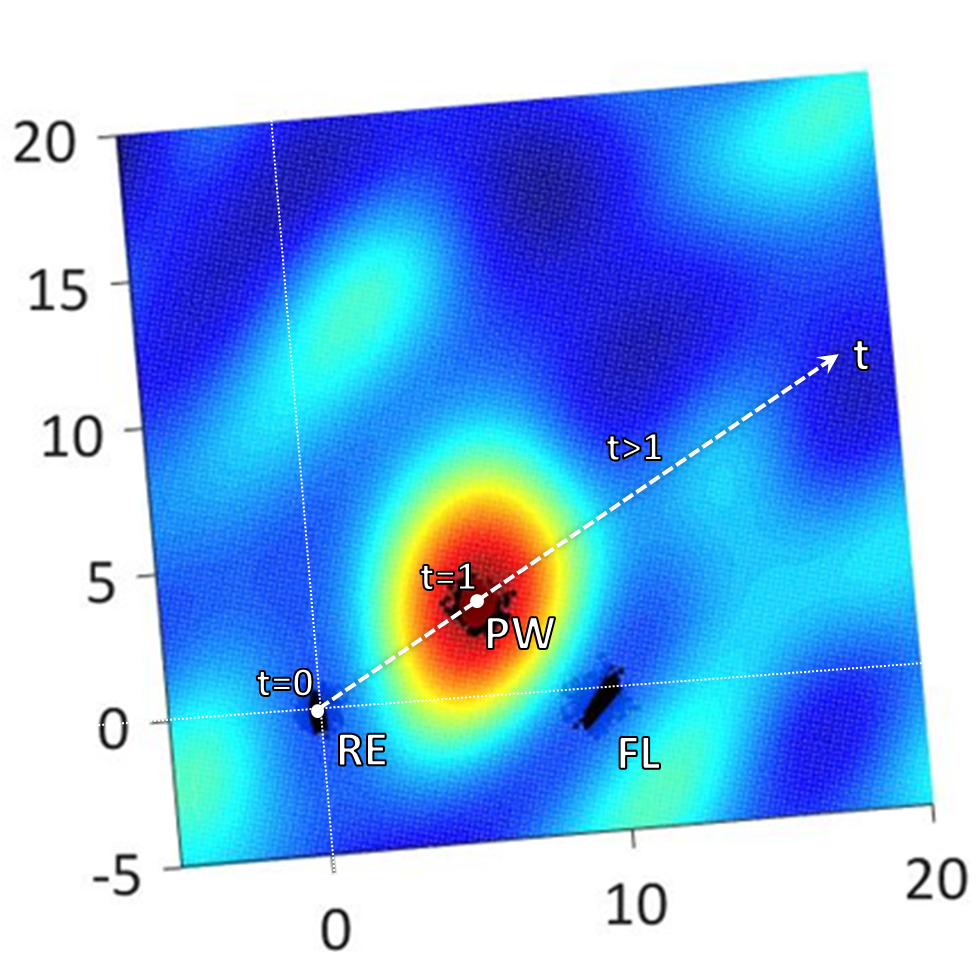
\includegraphics[width=0.8\textwidth]{Images/heatmap_DOF1.png}
    \caption{A 2D-reduced exemplary dataset S, obtained after gathering observations for three actions (black dots; rest, RE; power grasp, PW; wrist flexion, FL); the colour of the heat map denotes the value of the target value for power grasping, $f_{PW}$ . Values of the input space lying on the straight line $\overline{RE} + (\overline{PW} - \overline{RE})t_{PW}$ roughly denote power grasping with increasing strength.}
    \label{fig:heatmap}
\end{figure}
We define as $\overline{RE}$, $\overline{PW}$, $\overline{FL}$ the centers of the clusters corresponding respectively to the actions rest, power grasp and wrist flexion. In the figure is possible to see, as an heatmap, the function $f_{PW}$ obtained by training the learning model seen in section \ref{sec:ML} using the training set S.  
We decided to assume the straight line of the type $\overline{RE} + (\overline{PW} - \overline{RE})t_{PW}$ as the zone of the input space along which the participants signals move when she increase or decrease the force applied to a certain action; this assumption is justified by the physiology of the muscular activation and by our experimental observation.
As can be seen in figure \ref{fig:heatmap} between $t_{PW} = 0$ and $t_{PW} = 1$ the behaviour of the model is what we expected: the value of $f_{PW}$ increase with $t_{PW}$ and assume the maximum value for $t_{PW} = 1$, which corresponds to $\overline{PW}$. The problem become clear for the values of $t_{PW}$ greater than 1: almost immediately $f_{PW}$ begin to decrease and reaches 0 for $t_{PW} \approx 2$. In practice, the participant tries to apply more force and instead the hand open up, leading to drop the grasped object. This kind of failure is what we have called overshooting.
We are now able to give a formal definition of a model subject to overshooting:
\begin{equation}
    \exists A,t_A>1 : x = \overline{RE} + (\overline{A} - \overline{RE})t_{A} \implies f_A(x) < A_{max}
    \label{eq:overshooting}
\end{equation}
where $A$ indicates a general action on which we have trained the model and $A_{max}$ is the maximum activation value for that action. The other quantities correspond to what we have seen before but for a general action $A$.
Obviously the muscular activation in reality is not as precise and constant as we have supposed, therefore it will deviates from the straight line $\overline{RE} + (\overline{A} - \overline{RE})t_{A}$ and, as consequence, our definition of model subject to overshooting doesn't represent all the possible instances of overshooting. Nonetheless, thanks to the continuity of the nonlinear model we have chosen (RR-RFF sec. \ref{sec:ML}), the automated mending process manages to overall enhance the reliability of the system with respect to overshooting.
Overshooting can probably be defined in other ways, nevertheless we prefer to stick with the definition given in equation \ref{eq:overshooting} in order to limit as much as possible the subset of the input space we need to analyse to guarantee the absence of overshooting.
%
%
%
\section{Automated Procedure}
After having formally defined the overshooting problem we studied how to design an automated procedures which could bring the model to a state in which it wasn't subject to our definition of overshooting. In order to do so without changing drastically the structure of the learning model and of Interactive Myocontrol we decided to follow in the step of \cite{Strazzulla2017} and leverage the incrementality of the learning model used by Interactive Myocontrol.
The general idea of our automated procedure is to generate synthetic labelled samples which are then added to the original training set in order to modify the model and bring it in a state in which it is not subject to overshooting. With equation \ref{eq:overshooting} we have already given a preliminary definition of point in the input space which are affected by overshooting, it is reasonable to consider the above mentioned points as the one we are interested to add to the training set in order to modify the model so that they present the correct labels (e.g. they are no more subject to overshooting).
In general the idea of identify unsafe points and add them to a learning system in order to solve its vulnerability is extremely similiar to the adversarial learning methods presented in \cite{goodfellow2014generative}. The main differences is that in our case the adversary is not another learning model and we are not really in a security critical domain: we don't use the adversary in order to counter possible real-world security risk but just to explore a subset of interest of the input space.  
In order to preserve the coherence of the learning method we decided to keep the way we add points to the training set as similar as possible to the way the original training points are gathered: as seen before the training data are distributed in clusters corresponding to the different actions, therefore also our synthetic data will be distributed in the same way.
Given the characteristic of the training model and the possible interaction between the different actions, we decided to design our automated repair procedure as a iterative one:
\begin{enumerate}
    \item For each action of interest we search for an unsafe point (e.g. a point subject to overshooting, see equation \ref{eq:overshooting}), if no unsafe point is found for every action then the repair process is completed successfully.
    \item For each action for which we have found an unsafe point we generate a cluster centred on the point and we associate each point of the cluster with an appropriate label, then we add the point generated to the training set. We do nothing for the action for which we haven't found an unsafe point.
    \item The learning model is trained again but this time on the modified training set, then we continue with point 1.
\end{enumerate}
Obviously we still need to decide how to determine the appropriate label for the points we add to the training set: the natural choice appears to be the value $A_{max}$ seen in equation \ref{eq:overshooting} but experimentally we have found out that this kind of choice brings the repair procedure to need a longer time, and more unsafe points, in order to completely repair the model. This result is quite easy to understand: if our \textit{unsafety} condition is defined by equations \ref{eq:overshooting} we want that to every points $x = \overline{RE} + (\overline{A} - \overline{RE})t_{A}$ with $t_{A} >= 1$ corresponds a target value $f_A(x) >= A_{max}$ and if we consider the continuity of the learning model we have chosen, the adding of points with synthetic target value equals to $A_{max}$ it's unlikely to drastically modify the original model. Moreover from a theoretical point of view we would expect that to greater values of the input signals would correspond a greater activation level of the action. Therefore we chose as activation level for each synthetic point $x$ a value given by the following equation:
\begin{equation}
    y_{syn} = y_0 + c_A \cdot (x_{proj} - \overline{RE})
    \label{eq:output_unsafe}
\end{equation}
where $c_A$ is the slope of the straight line connecting $(\overline{RE}, 0)$ and $(\overline{A}, A_{max})$ in the space $\mathbb{R}^9$ (e.g. remember that the input space is $\mathbb{R}^8$ and the activation value is a real number), $x_{proj}$ is the projection of the point $x$ on the straight line $\overline{RE} + (\overline{A} - \overline{RE})t_{A}$ and $y_0$ is a quantity we have determined experimentally.
For what concern the generation of the clusters we have chosen to draw the points from a normal distribution with mean equals to the original unsafe point and variance equals to the variance of the cluster generated during the training corresponding to the action of interest. The number of points drawn is equal to the number of point of the original cluster.
The last problem we need to solve before being able to implement our automated repair process is how we can find the unsafe points: in this thesis we have studied two different methods to do so.
The first method we have considered use an SMT solver in order to search for unsafe points: the problem is encoded as a propositional logic formula and then the SMT solver is used to find a solution of such formula, in equation \ref{eq:SMT-formula} we show the logic formula we give to the SMT solver.
\begin{equation}
\begin{aligned}
    t \geq t_{min} \wedge t \leq t_{max}\qquad \wedge \\
    \mathbf{\phi}(t) = cos(\sigma \cdot \mathbf{\Omega} \cdot (\overline{RE} + (\overline{A} - \overline{RE})t)\qquad \wedge \\
    y = \mathbf{w}^T \phi(t)\qquad \wedge \\
    y < A_{max}\qquad\quad
    \label{eq:SMT-formula}
\end{aligned}
\end{equation}
where $t_{min}$ and $t_{max}$ define the interval of the straight line we are interested in and the other quantities are the same we have defined in the previous sections. The main difference from the learning model seen in section \ref{sec:ML} is that we have $\phi(t)$ instead of $\phi(\mathbf{x})$: actually there is no real difference, we have only highlighted the dependence from the variable t. Changing the dependence from $\mathbf{x}$ to only $t$ radically simplify the work of the SMT solver: the space it needs to analyse goes from $\mathbb{R}^8$ to just $\mathbb{R}$. This simplification is what make possible to use an SMT solver: in the preliminary test we have done, using a formulation of the problem which used $\mathbf{x}$ instead of $t$ as variable, the solver wasn't able to complete successfully the analysis due to the excessive computational complexity. We have called SMT-repair the repair process which uses this method to find the unsafe points.\\
The second method we have considered consists in generating a set of point uniformly distributed along the straight line corresponding to the action of interest, computing their target values and analysing them in order to find one that doesn't respect the safety condition. In this case we are able to search for \textit{the unsafest} point, e.g. the point $\mathbf{x}$ which maximise the quantity $A_{max} - f(\mathbf{x})$. We have called PDO-Repair the repair process which uses this method to find the unsafe points.\\
At this point we have managed to design all the parts of the automated procedure, therefore we just need to put them together. Below we show a pseudocode of our procedure:
\vspace{5mm}\small
\begin{algorithmic}
	\STATE $\mathbf{w} \gets \mathbf{buildModel}(S)$
	\STATE $unsafe \gets True$
	\WHILE{$unsafe$}
	\FOR{\textbf{each action} $A$}
	\STATE [$unsafe$ ,$t_A^U$] $\gets \mathbf{safetyCheck}(\mathbf{w}, S)$
	\IF{$unsafe$}
	\STATE $(X',Y') \gets (\mathcal{N}(t_A^U,\sigma_A),\mathbf{y}_A)$
	\STATE $\mathbf{w} \gets \mathbf{buildModel}(S \cup (X',Y'))$
	\ENDIF
	\ENDFOR
	\ENDWHILE
\end{algorithmic}
\vspace{5mm}\normalsize
In the pseudocode above the function $\mathbf{safetyCheck}(...)$ represent one of the two methods we have considered in this section and $\mathbf{buildModel}(...)$ represent the training of the learning model. In the following we show how the model change during the execution of the repair procedure for both the safety check methods.
\subsection{Execution of PDO-Repair}\label{subsec:PDO-Repair}
The following images show an example of an execution of the PDO-Repair on a training set which consider the actions: power grasp, wrist flexion and wrist extension. In particular we show the progress of the model along the straight lines we have considered during this section.
\begin{figure}[ht]
    \centering
    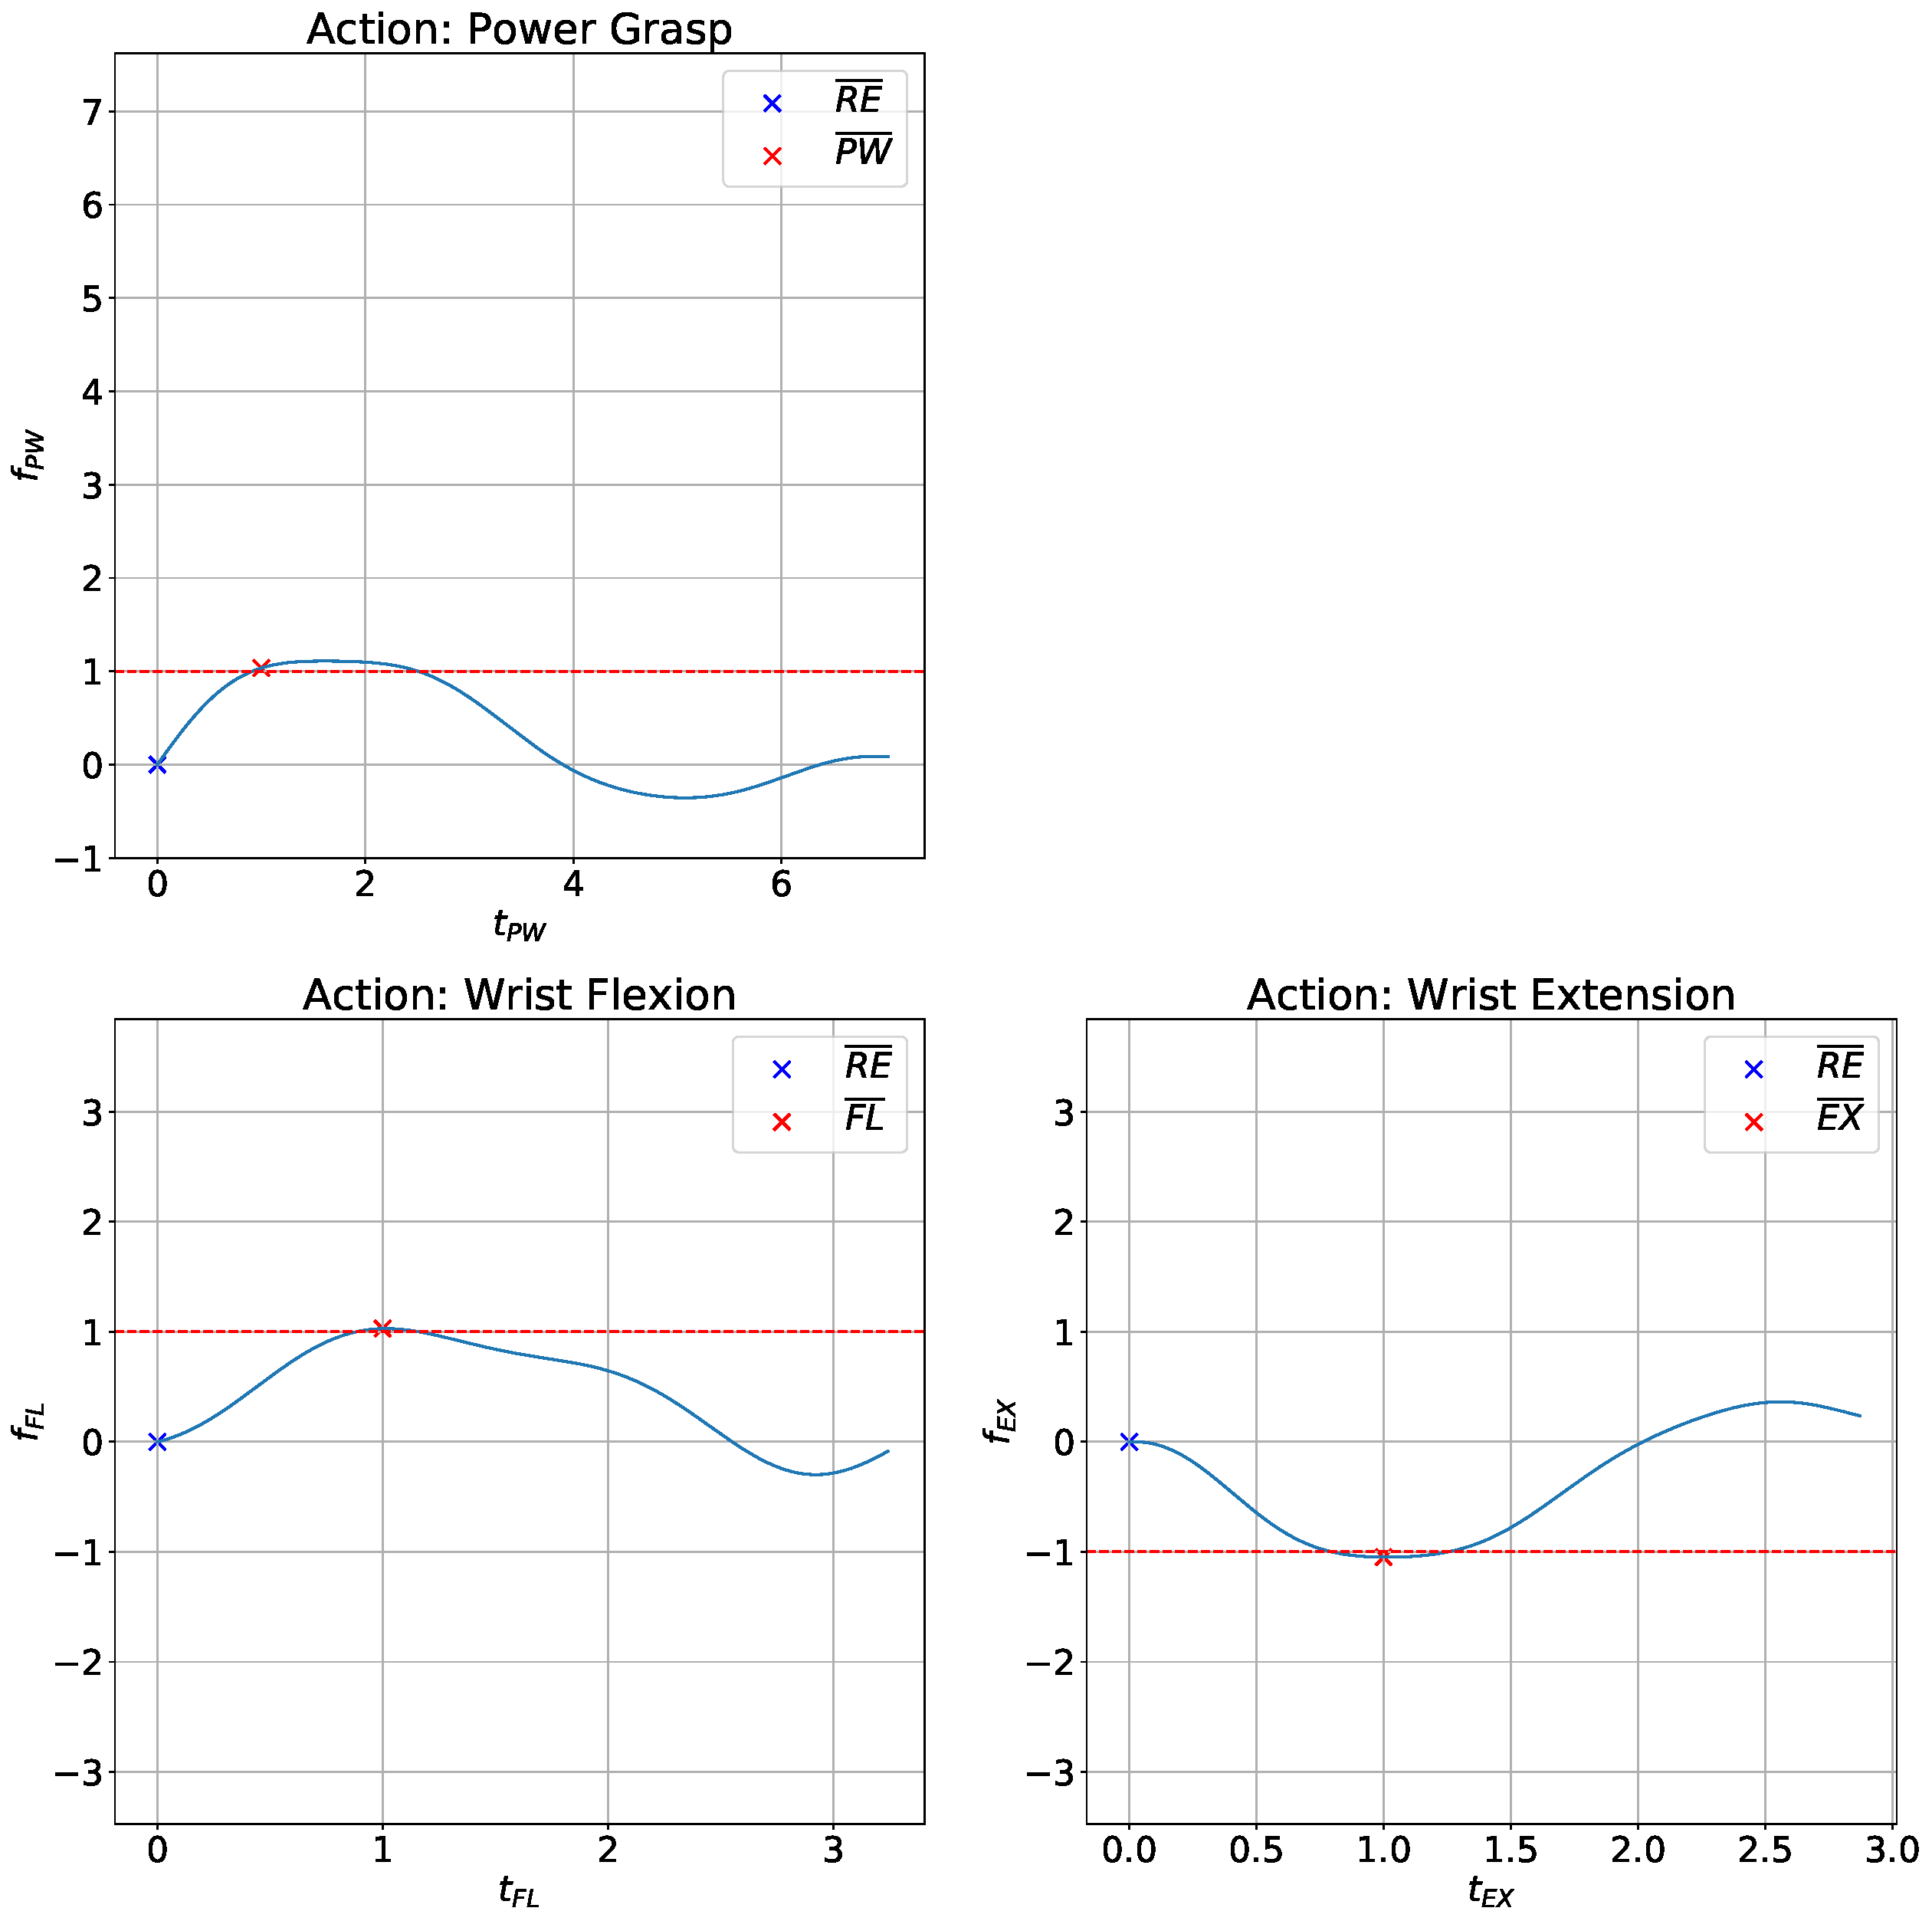
\includegraphics[width=\textwidth]{Images/repair-example/PDO-State0.pdf}
    \caption{In this figure we show the original model along the straight lines $\overline{RE} + (\overline{PW} - \overline{RE})t_{PW}$, $\overline{RE} + (\overline{FL} - \overline{RE})t_{FL}$ and $\overline{RE} + (\overline{EX} - \overline{RE})t_{EX}$. As can be seen the model is subject to overshooting along all the three lines. The red dashed lines represent the maximum activation values for the different actions.}
    \label{fig:PDO-exec-0}
\end{figure}
It can be noted in figure \ref{fig:PDO-exec-0} that for the action $EX$ the target value is negative (to be precise $EX_{max} = 1$), this fact doesn't change what we have seen till now: the extension of the automated procedure to this case is trivial. The negative target value is due to the fact that $FL$ and $EX$ correspond to the same degree of freedom, therefore they present opposite activation value. The belonging to the same degree of freedom of the two actions is easily understood considering that they are physically mutually exclusive, e.g. it is impossible to flex and extend the wrist at the same time. Moreover, as far as we know, in all the prosthetic hand the two action are managed by the same actuator.
\begin{figure}[ht]
    \centering
    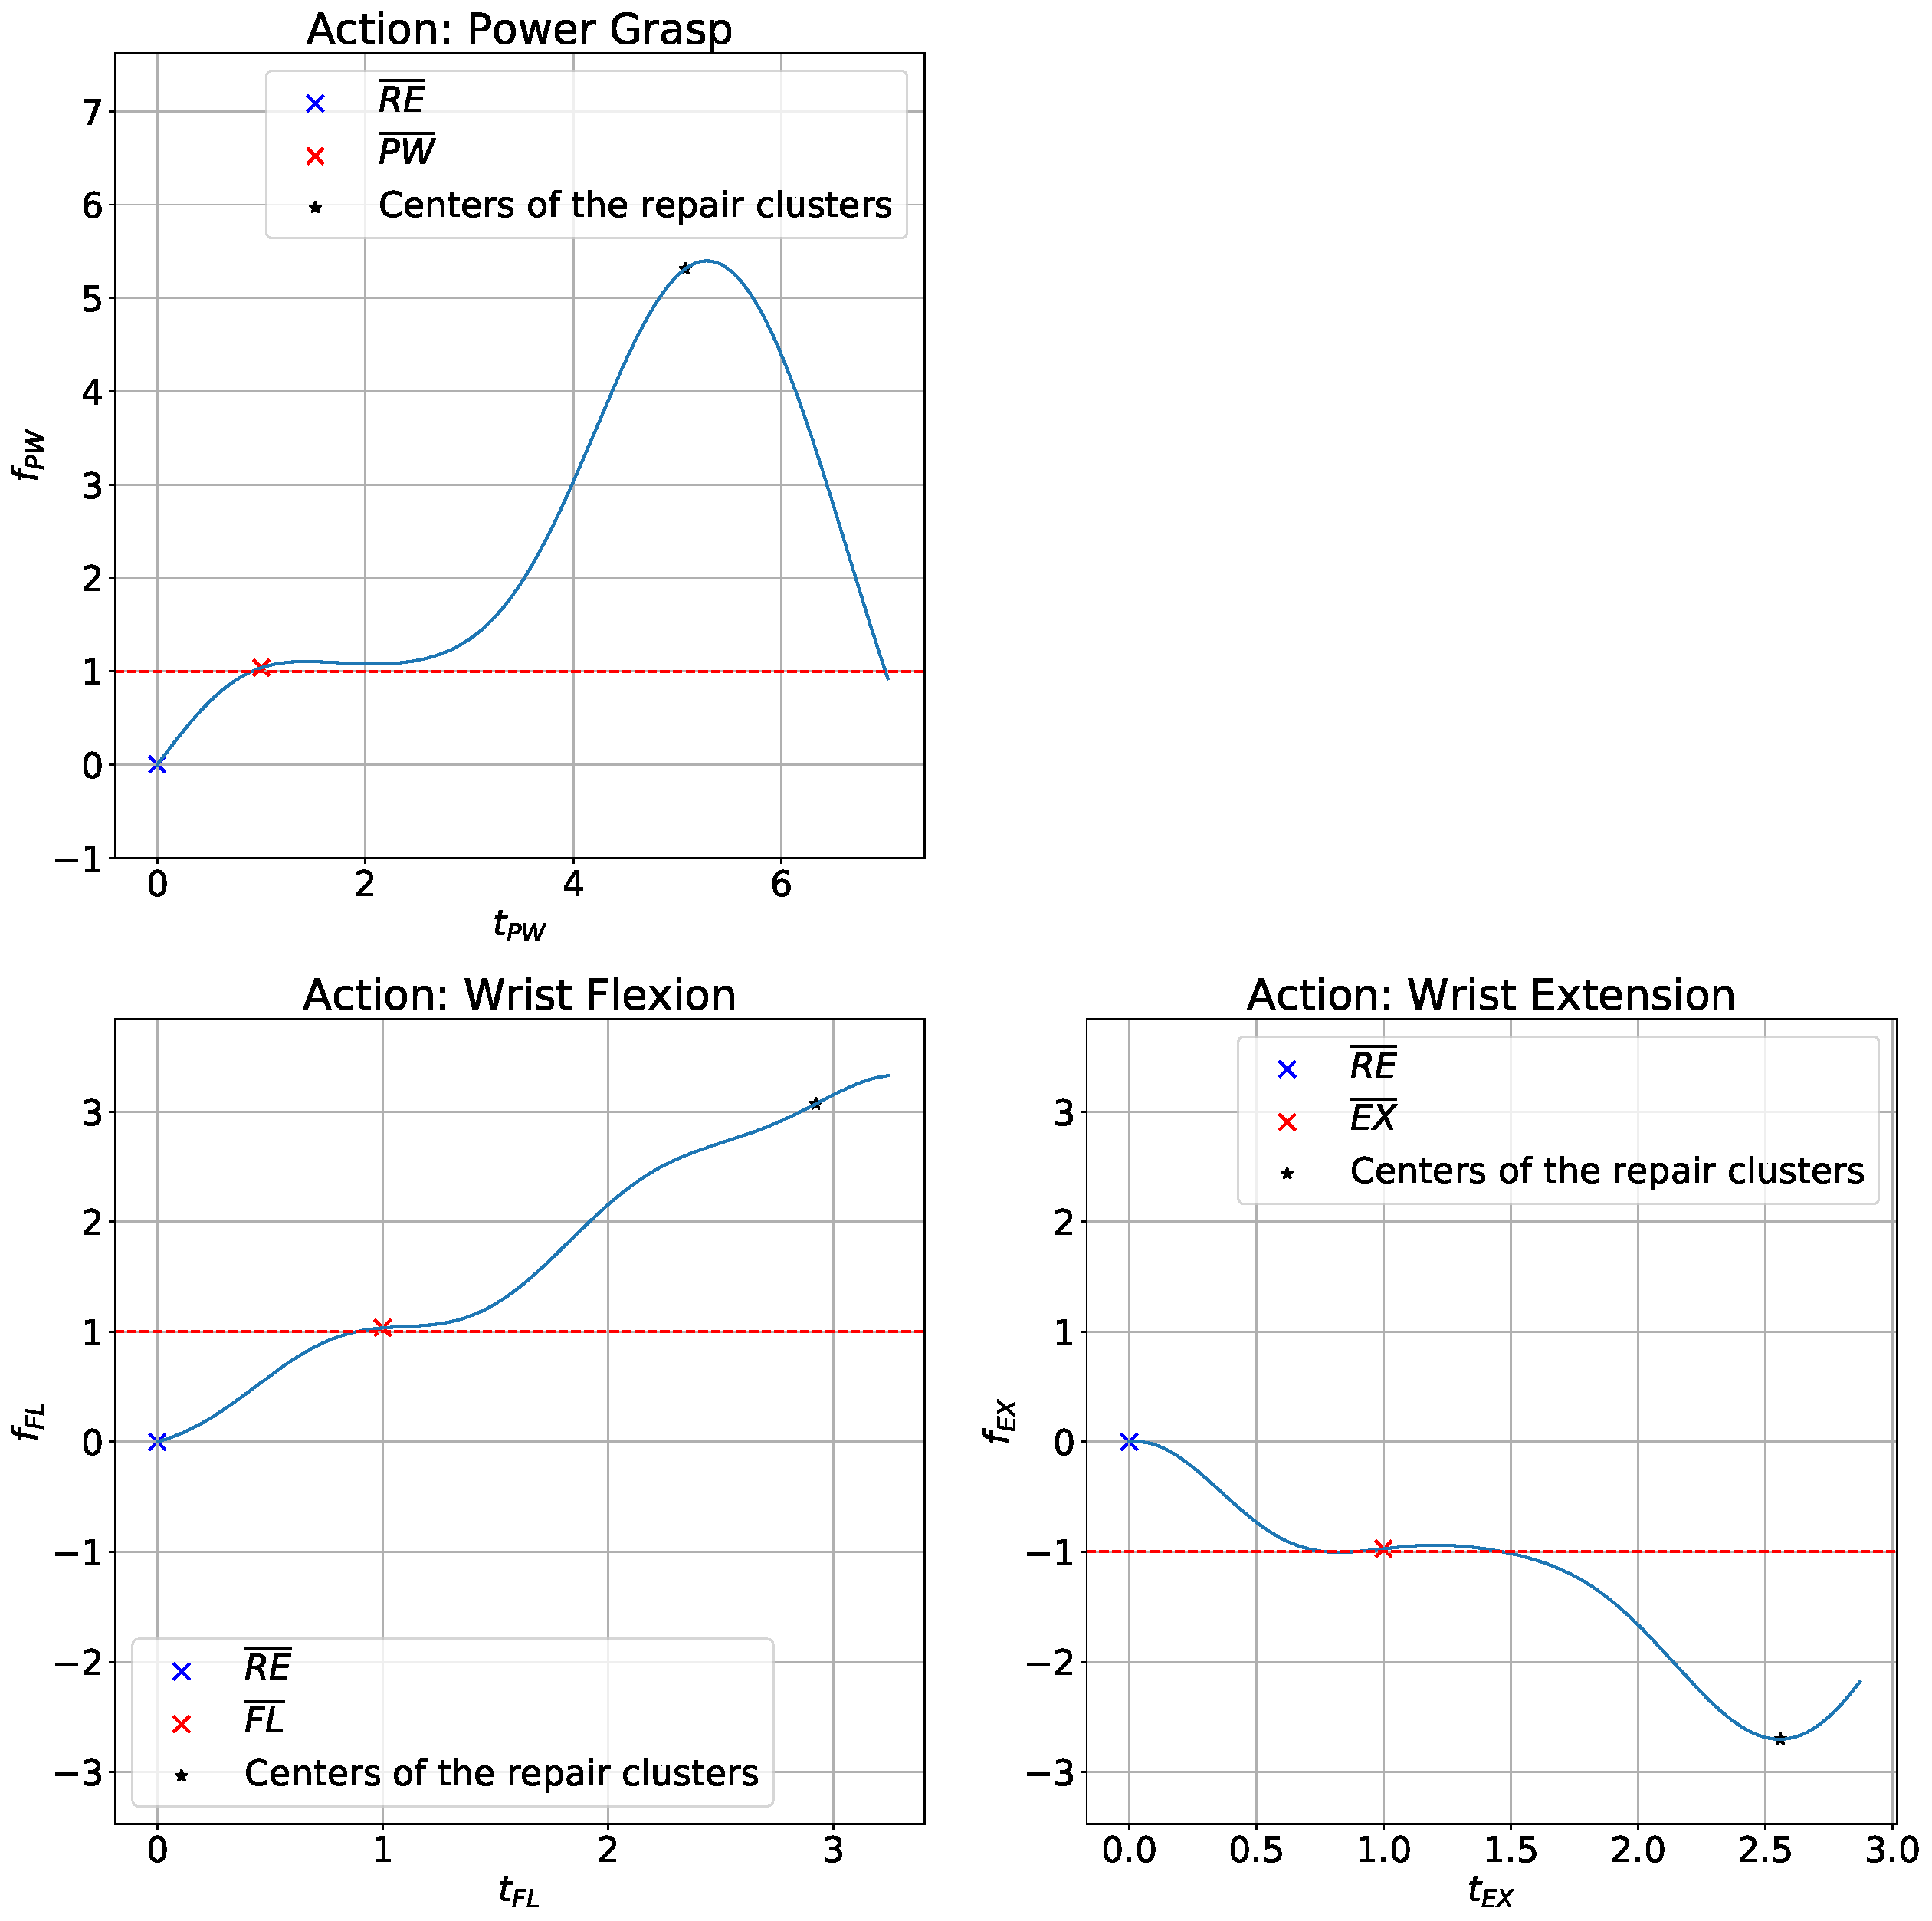
\includegraphics[width=\textwidth]{Images/repair-example/PDO-State1.pdf}
    \caption{In this figure we show the model along the straight lines $\overline{RE} + (\overline{PW} - \overline{RE})t_{PW}$, $\overline{RE} + (\overline{FL} - \overline{RE})t_{FL}$ and $\overline{RE} + (\overline{EX} - \overline{RE})t_{EX}$ after the first round of repair. The red dashed lines represent the maximum activation values for the different actions.}
    \label{fig:PDO-exec-1}
\end{figure}
Comparing figures \ref{fig:PDO-exec-1} and \ref{fig:PDO-exec-2} permits to see that the repair of the model along the straight lines is done only when it is needed: between the first and second iteration of the repair process there is no repair done along the straight line of the action $FL$, whereas the repair proceeds for the other two lines.
\begin{figure}[ht]
    \centering
    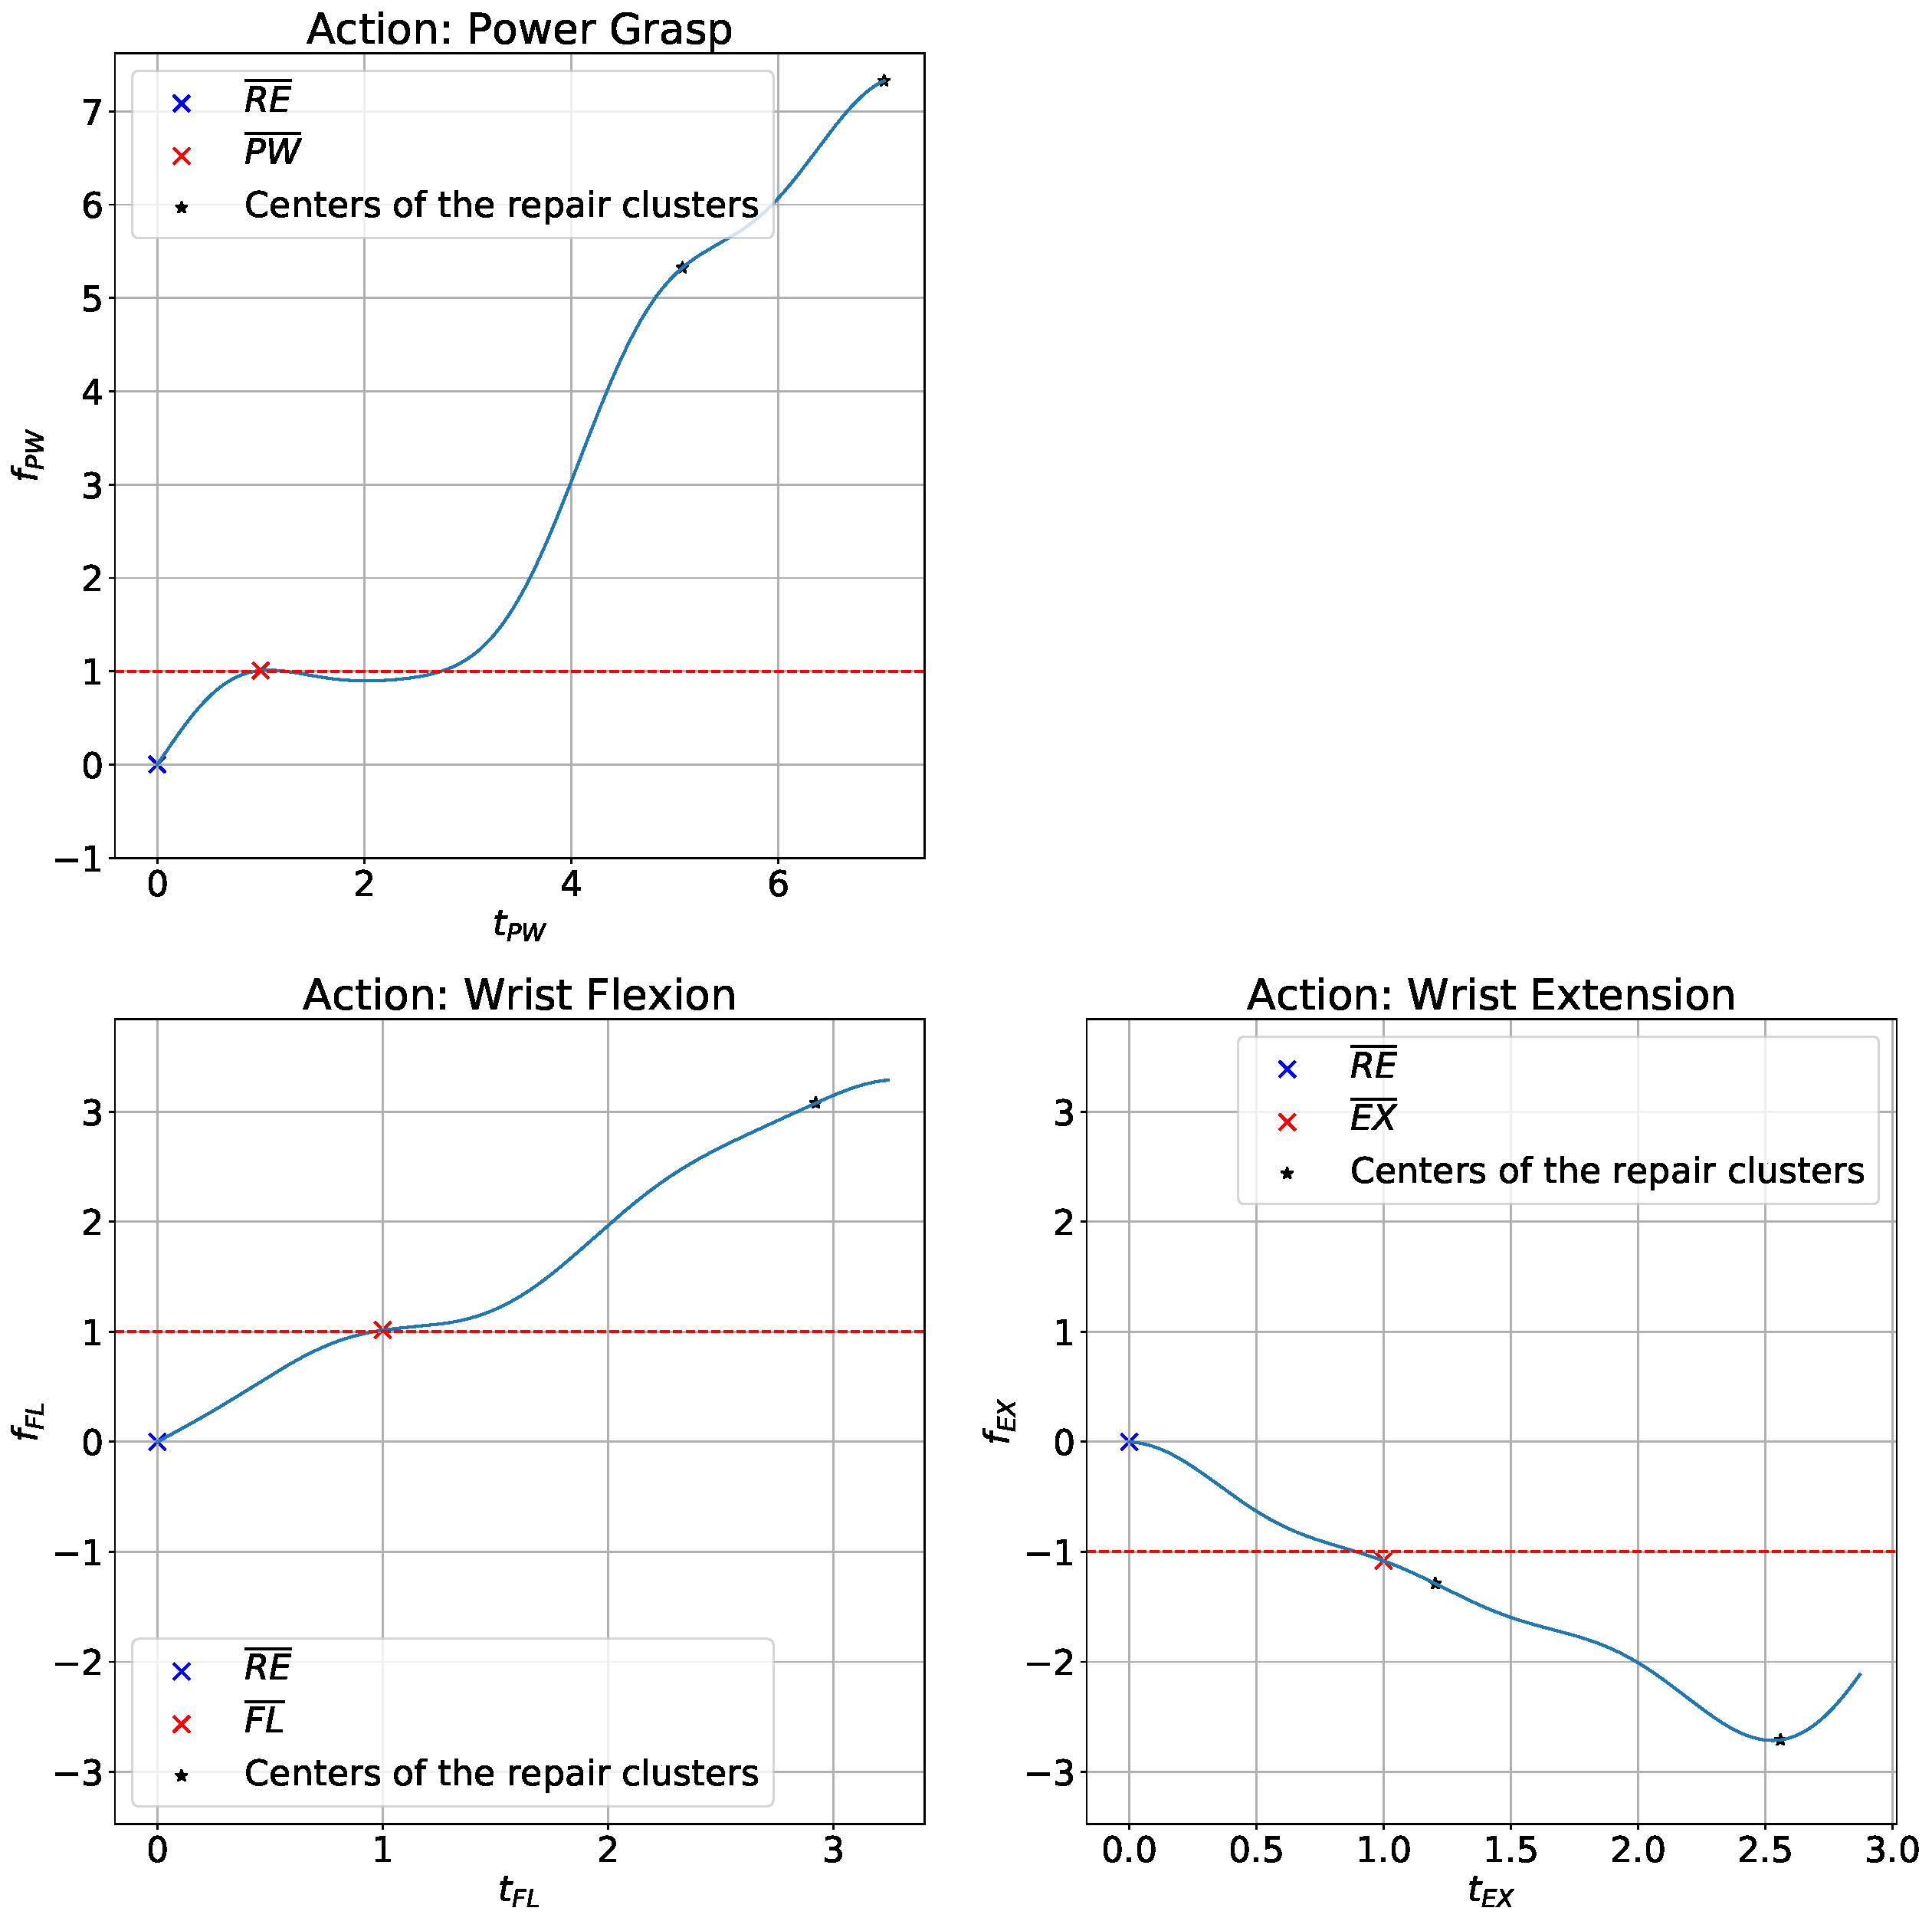
\includegraphics[width=\textwidth]{Images/repair-example/PDO-State2.pdf}
    \caption{In this figure we show the model along the straight lines $\overline{RE} + (\overline{PW} - \overline{RE})t_{PW}$, $\overline{RE} + (\overline{FL} - \overline{RE})t_{FL}$ and $\overline{RE} + (\overline{EX} - \overline{RE})t_{EX}$ after the second round of repair. The red dashed lines represent the maximum activation values for the different actions.}
    \label{fig:PDO-exec-2}
\end{figure}
It is also possible to see that, due to the characteristic of the learning model, the repair done in a particular point can bring to the appearance of unsafety in other points, therefore the necessity of an iterative repair procedure.
\begin{figure}[H]
    \centering
    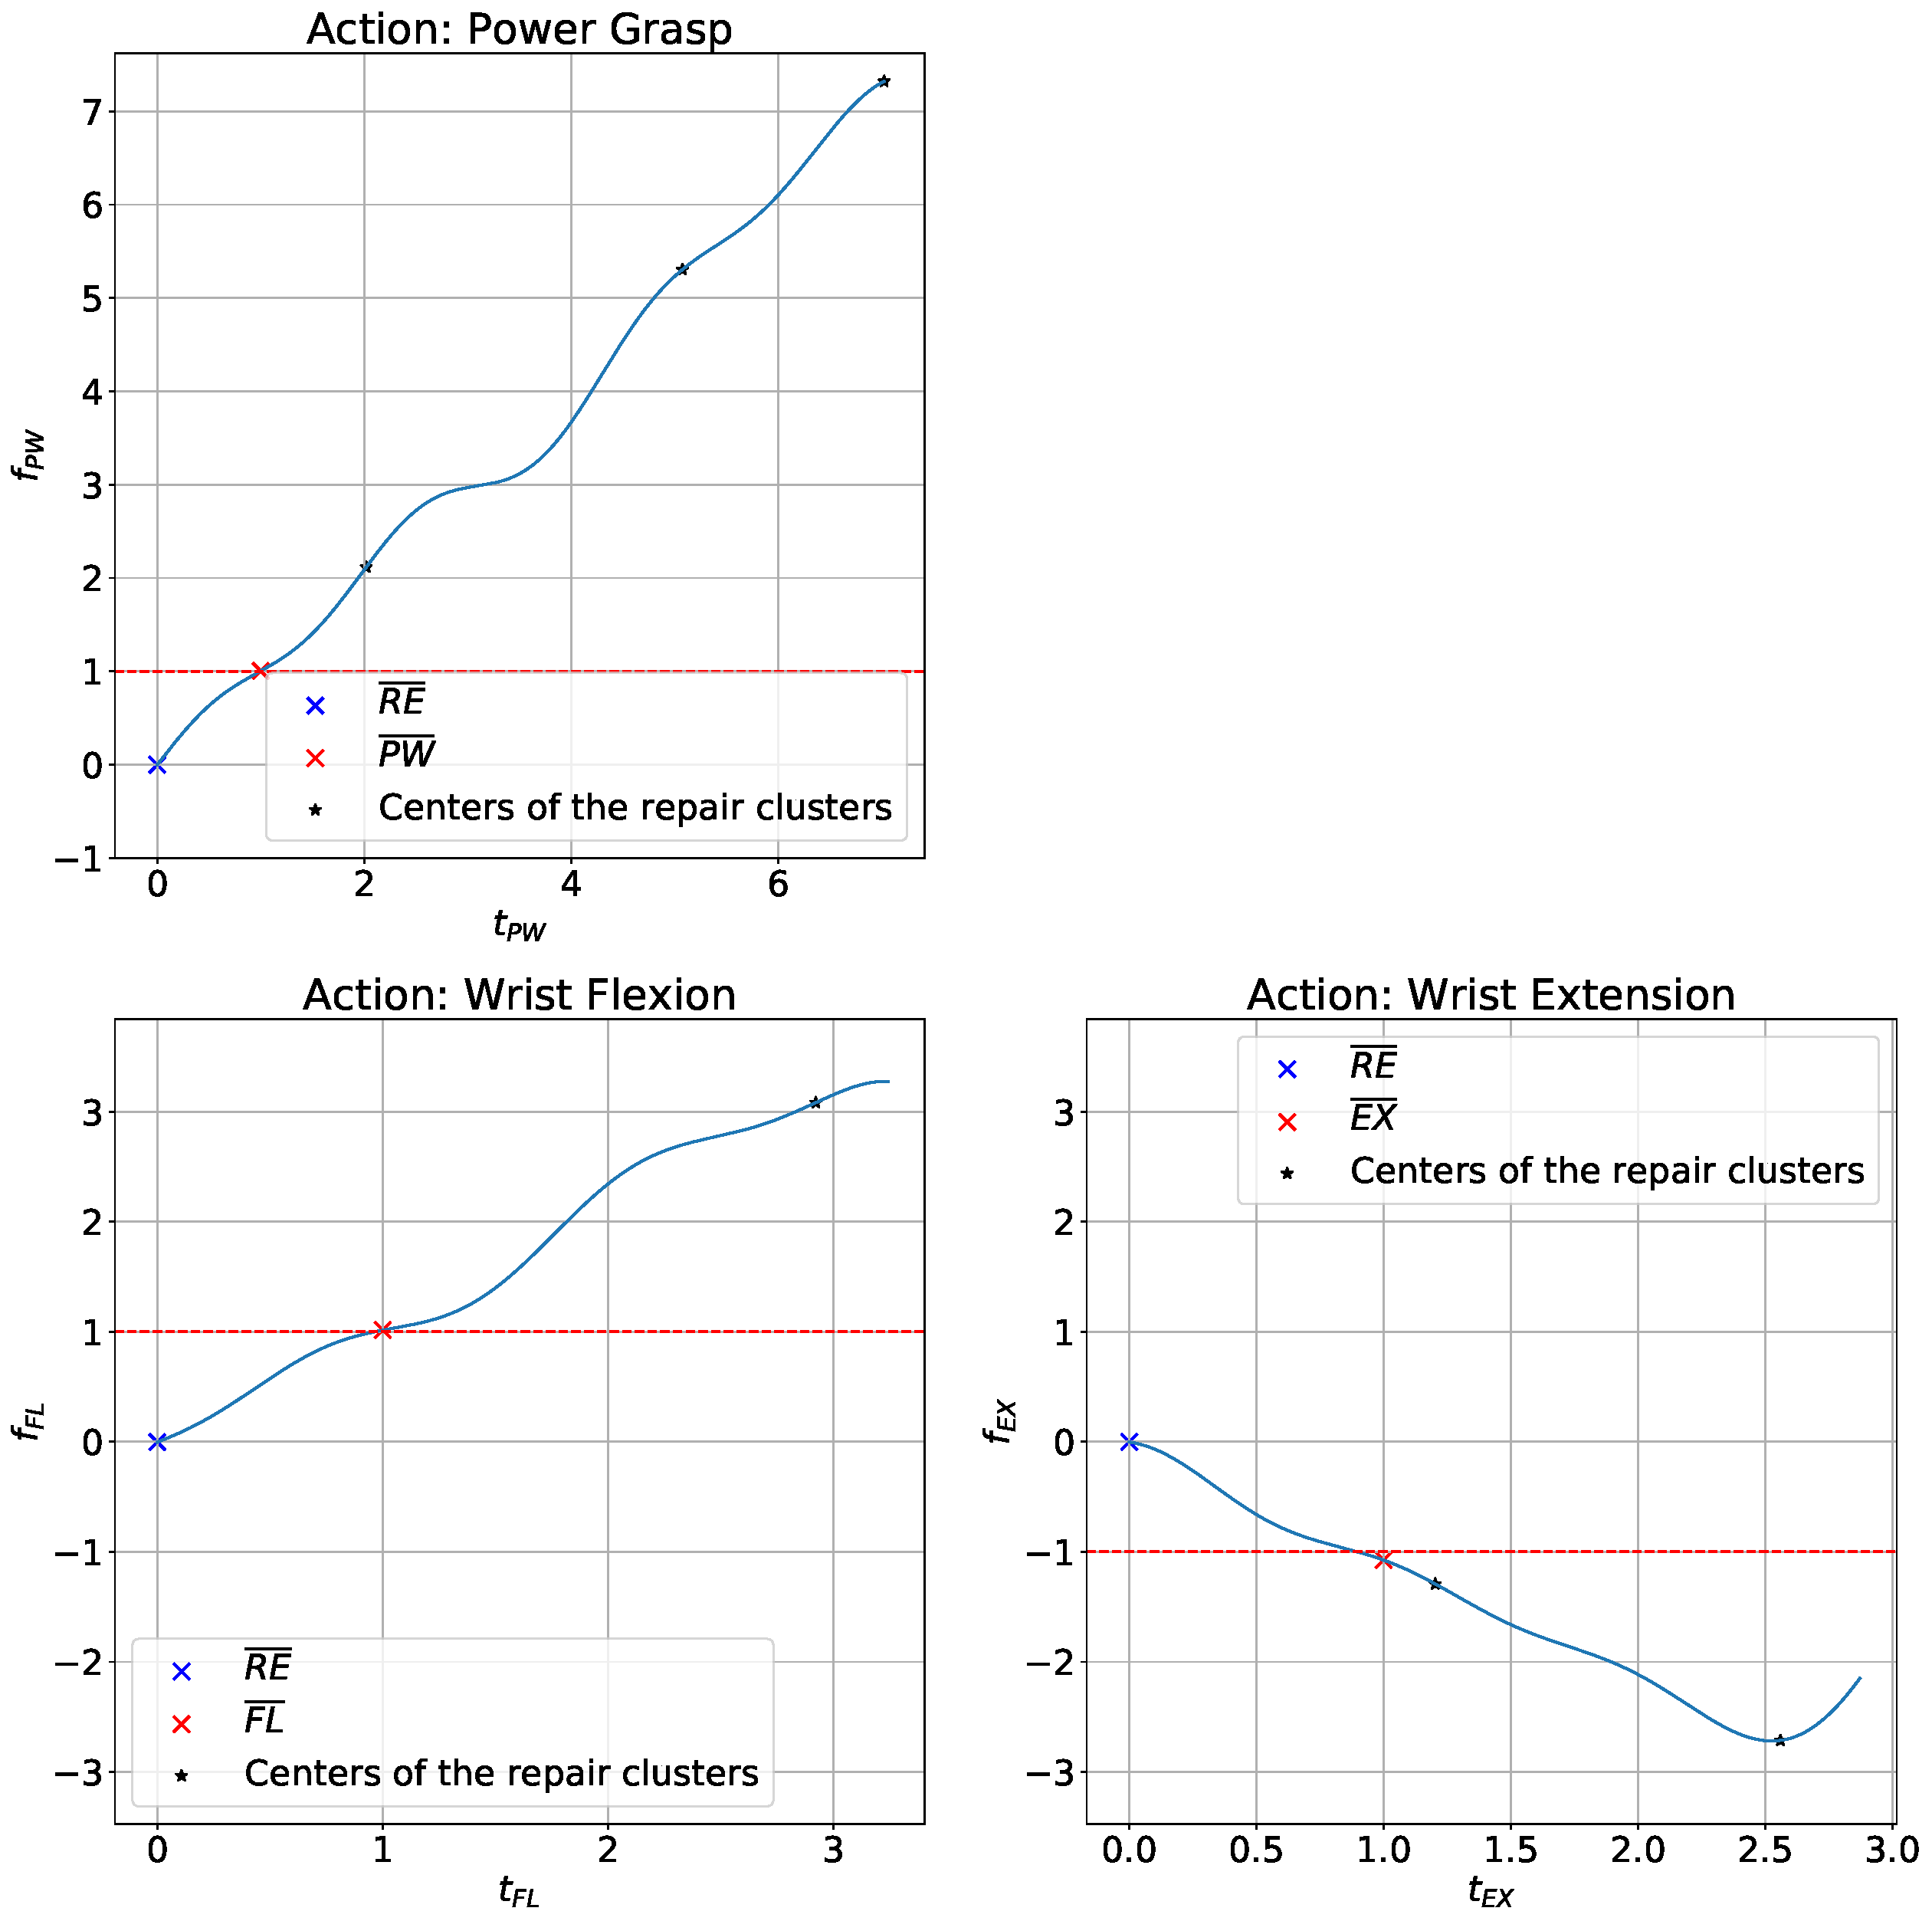
\includegraphics[width=\textwidth]{Images/repair-example/PDO-State3.pdf}
    \caption{In this figure we show the model along the straight lines $\overline{RE} + (\overline{PW} - \overline{RE})t_{PW}$, $\overline{RE} + (\overline{FL} - \overline{RE})t_{FL}$ and $\overline{RE} + (\overline{EX} - \overline{RE})t_{EX}$ after the final round of repair. The red dashed lines represent the maximum activation values for the different actions.}
    \label{fig:PDO-exec-3}
\end{figure}
As can be seen in figure \ref{fig:PDO-exec-3} the result of the repair process it is similar to a linearization of the functions $f_{PW}$, $f_{FL}$ and $f_{EX}$, which is quite reasonable: in general we would expect that to a linear increase in the muscular force applied would correspond a linear increase in the activation of a certain action.
%
%
\subsection{Execution of SMT-Repair}\label{subsec:SMT-Repair}
The following images show an example of an execution of the SMT-Repair on the same training set used for the example of the PDO-Repair.
\begin{figure}[H]
    \centering
    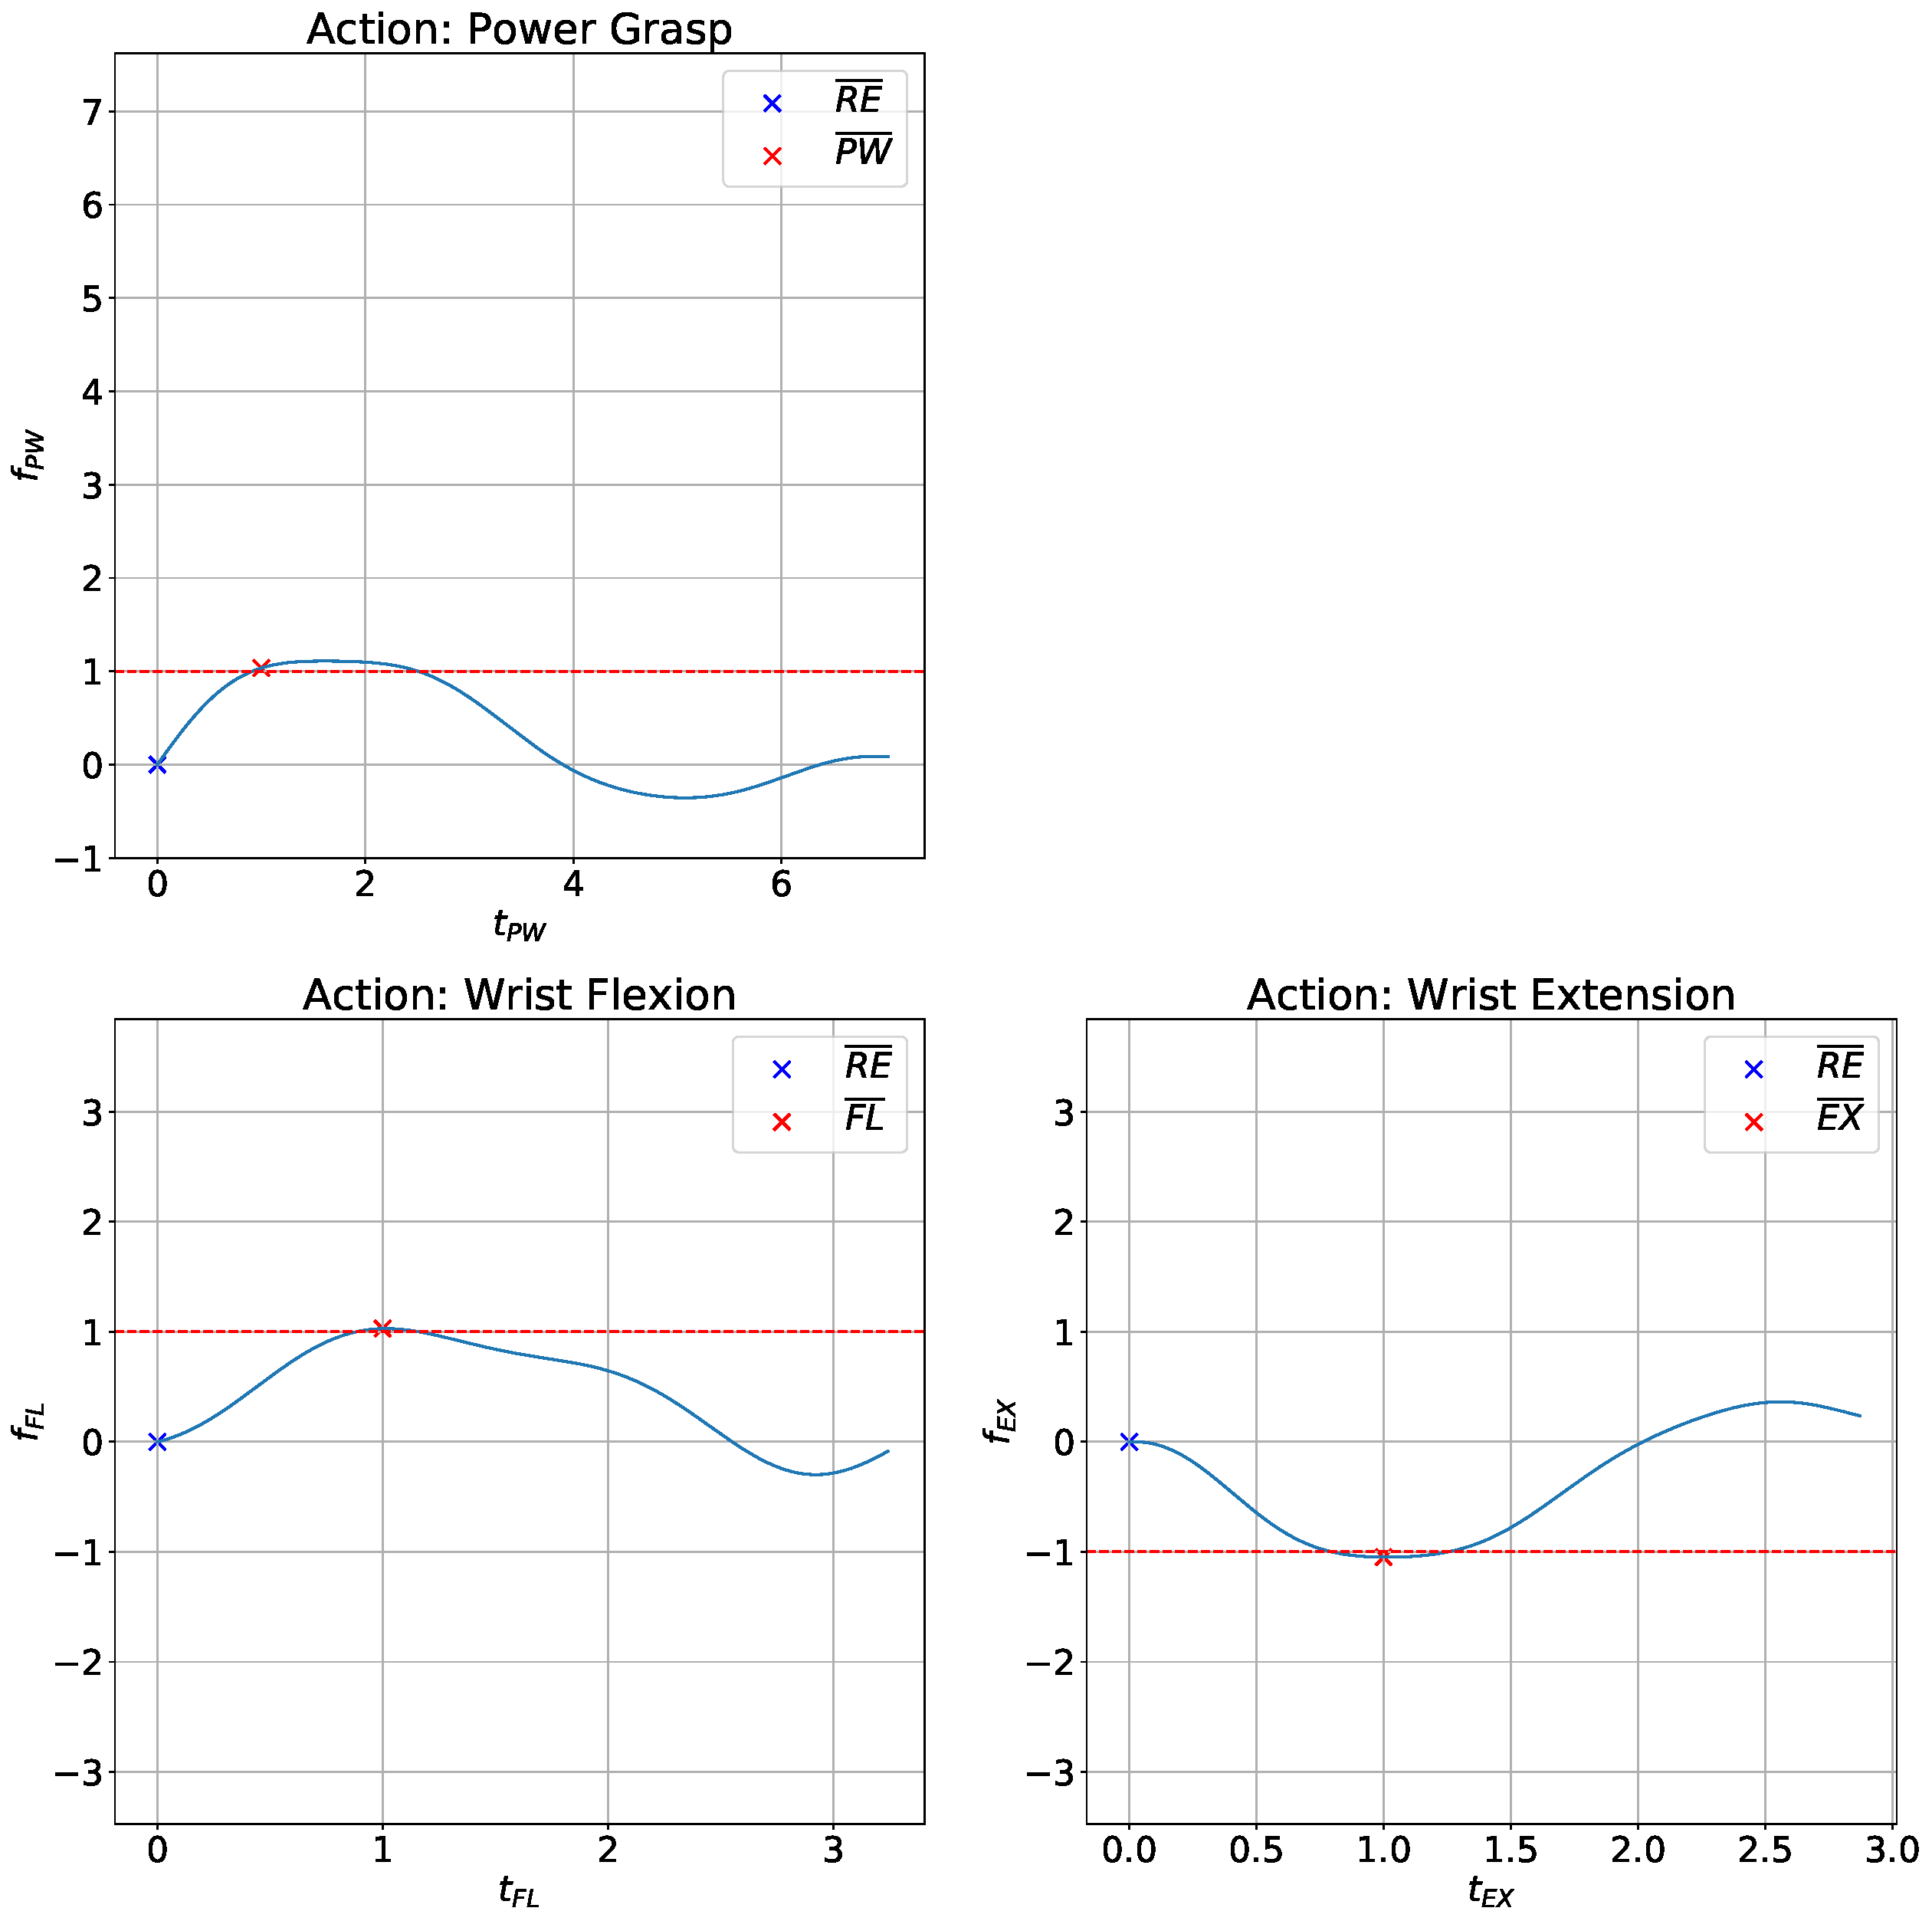
\includegraphics[width=\textwidth]{Images/repair-example/SMT-State0.pdf}
    \caption{In this figure we show the original model along the straight lines $\overline{RE} + (\overline{PW} - \overline{RE})t_{PW}$, $\overline{RE} + (\overline{FL} - \overline{RE})t_{FL}$ and $\overline{RE} + (\overline{EX} - \overline{RE})t_{EX}$. The red dashed lines represent the maximum activation values for the different actions.}
    \label{fig:SMT-exec-0}
\end{figure}
\begin{figure}[H]
    \centering
    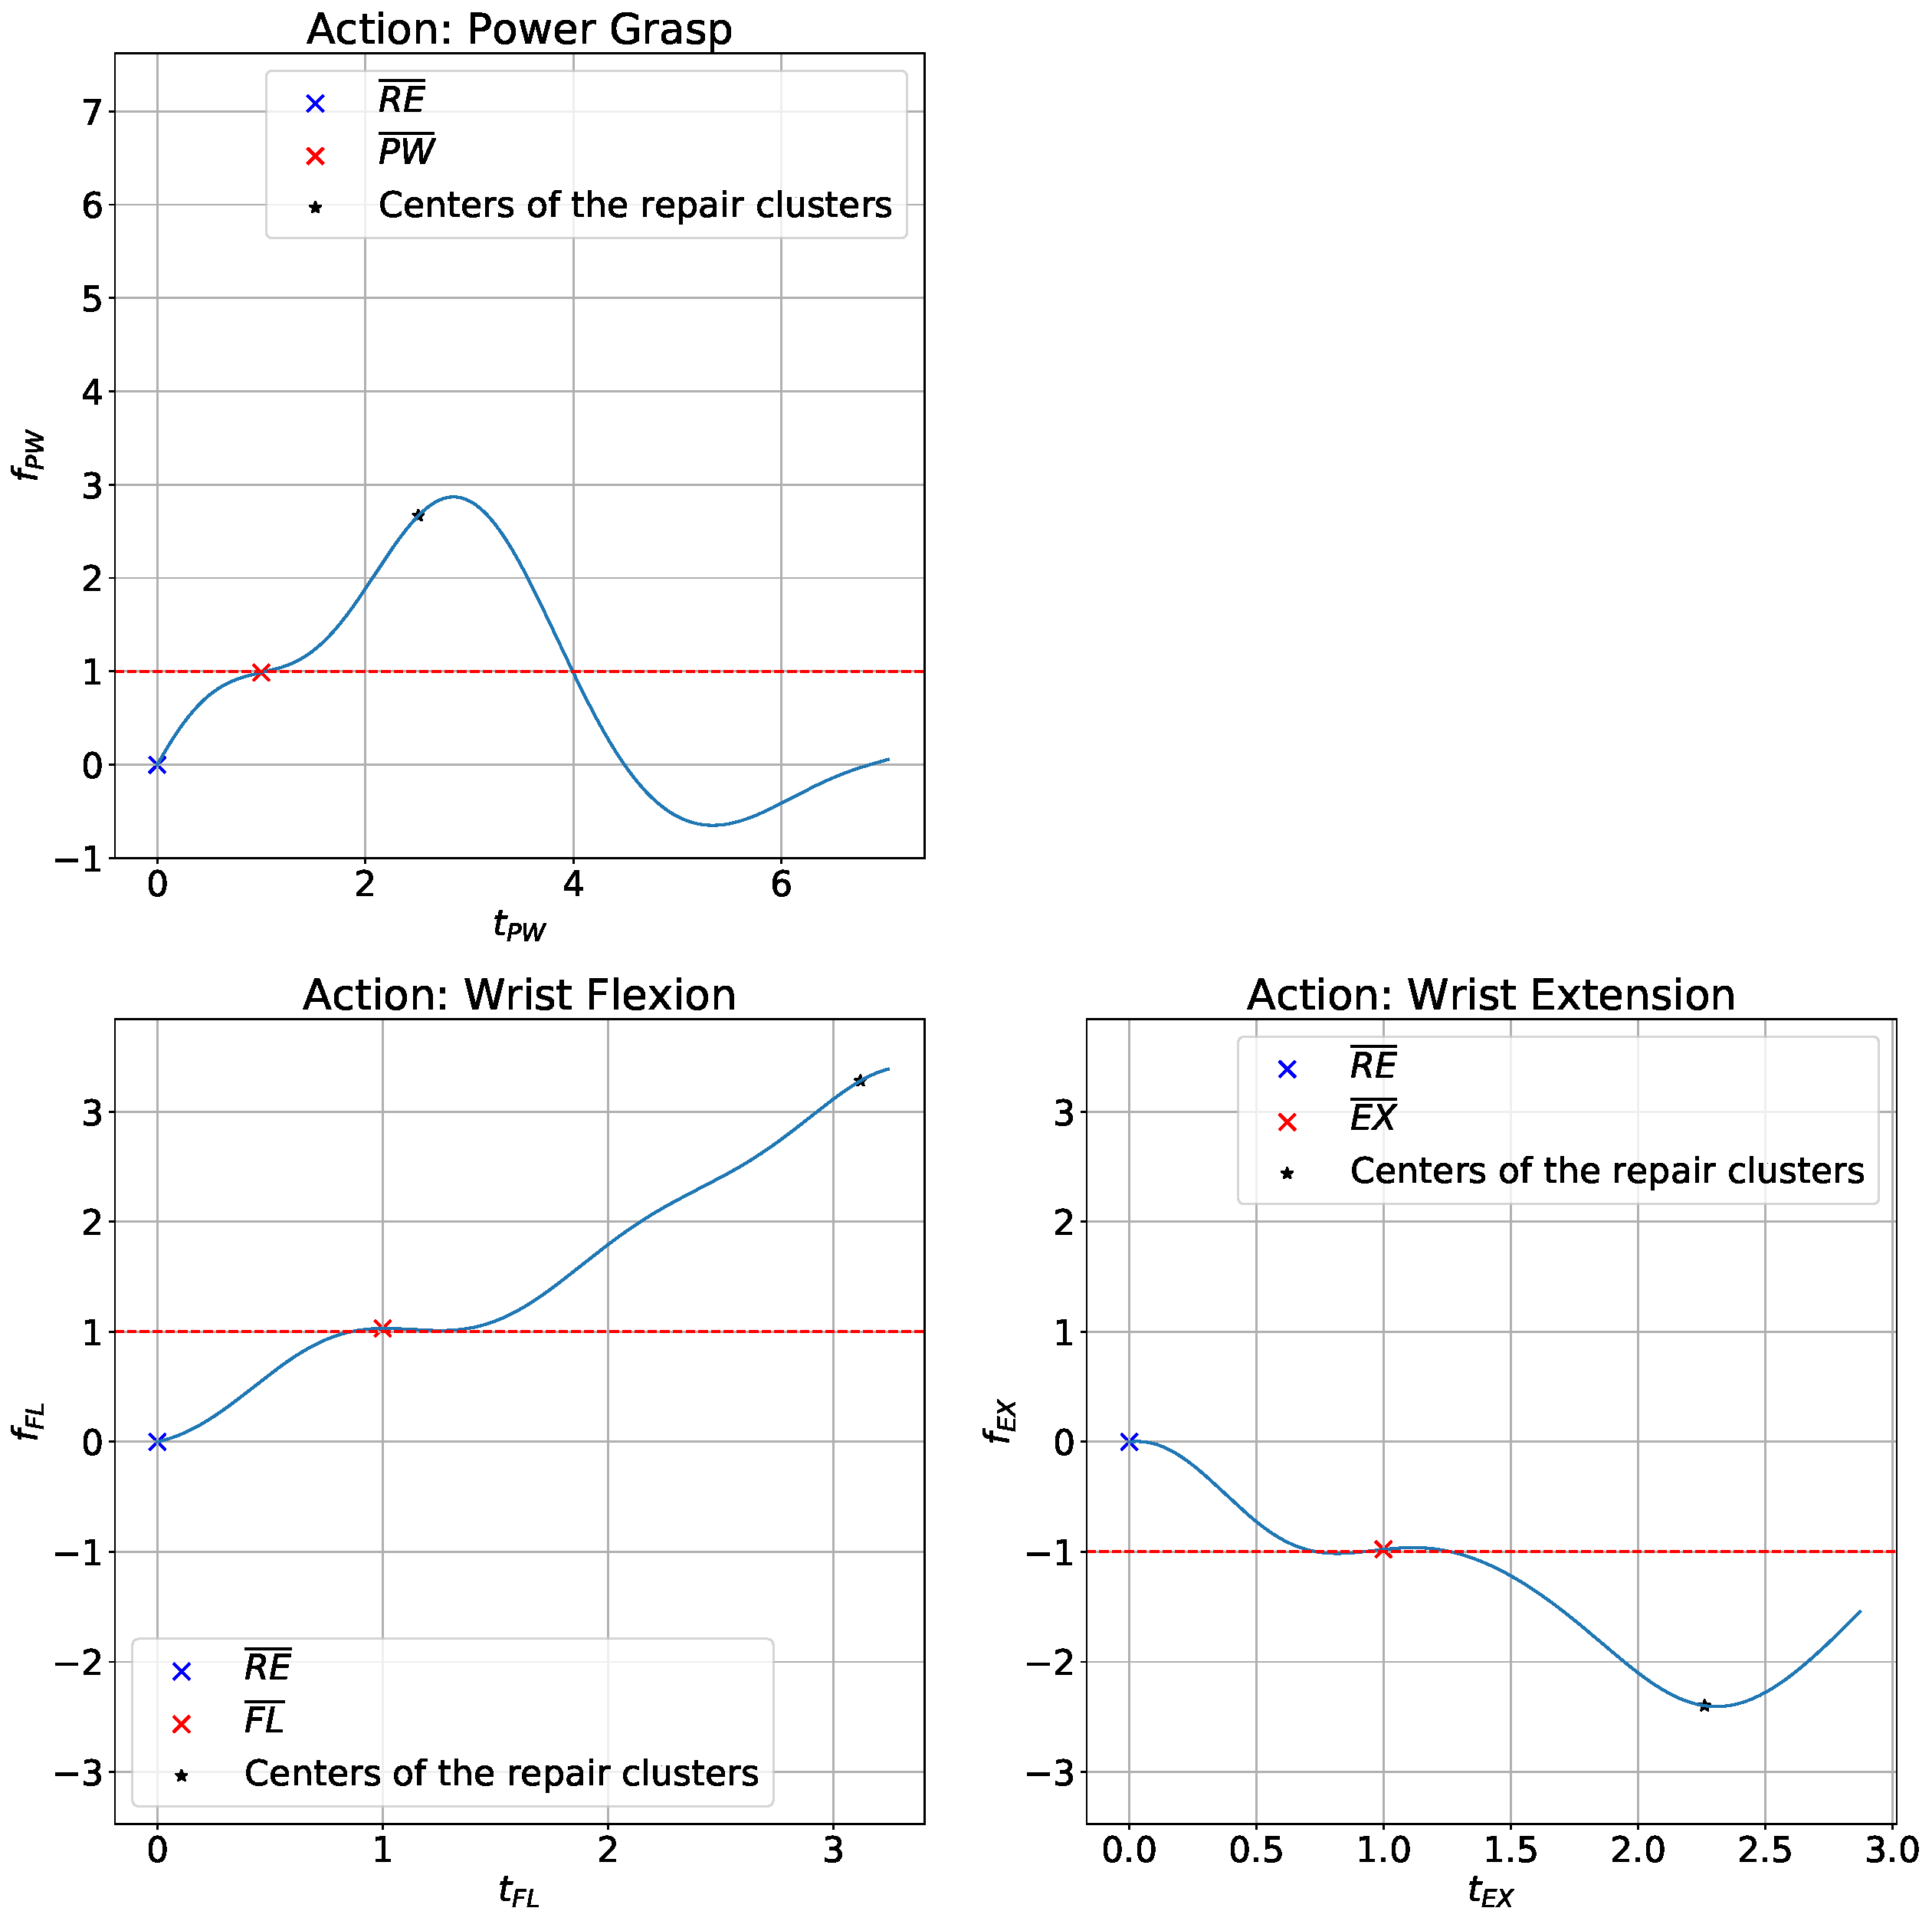
\includegraphics[width=\textwidth]{Images/repair-example/SMT-State1.pdf}
    \caption{In this figure we show the model along the straight lines $\overline{RE} + (\overline{PW} - \overline{RE})t_{PW}$, $\overline{RE} + (\overline{FL} - \overline{RE})t_{FL}$ and $\overline{RE} + (\overline{EX} - \overline{RE})t_{EX}$ after the first round of repair. The red dashed lines represent the maximum activation values for the different actions.}
    \label{fig:SMT-exec-1}
\end{figure}
\begin{figure}[H]
    \centering
    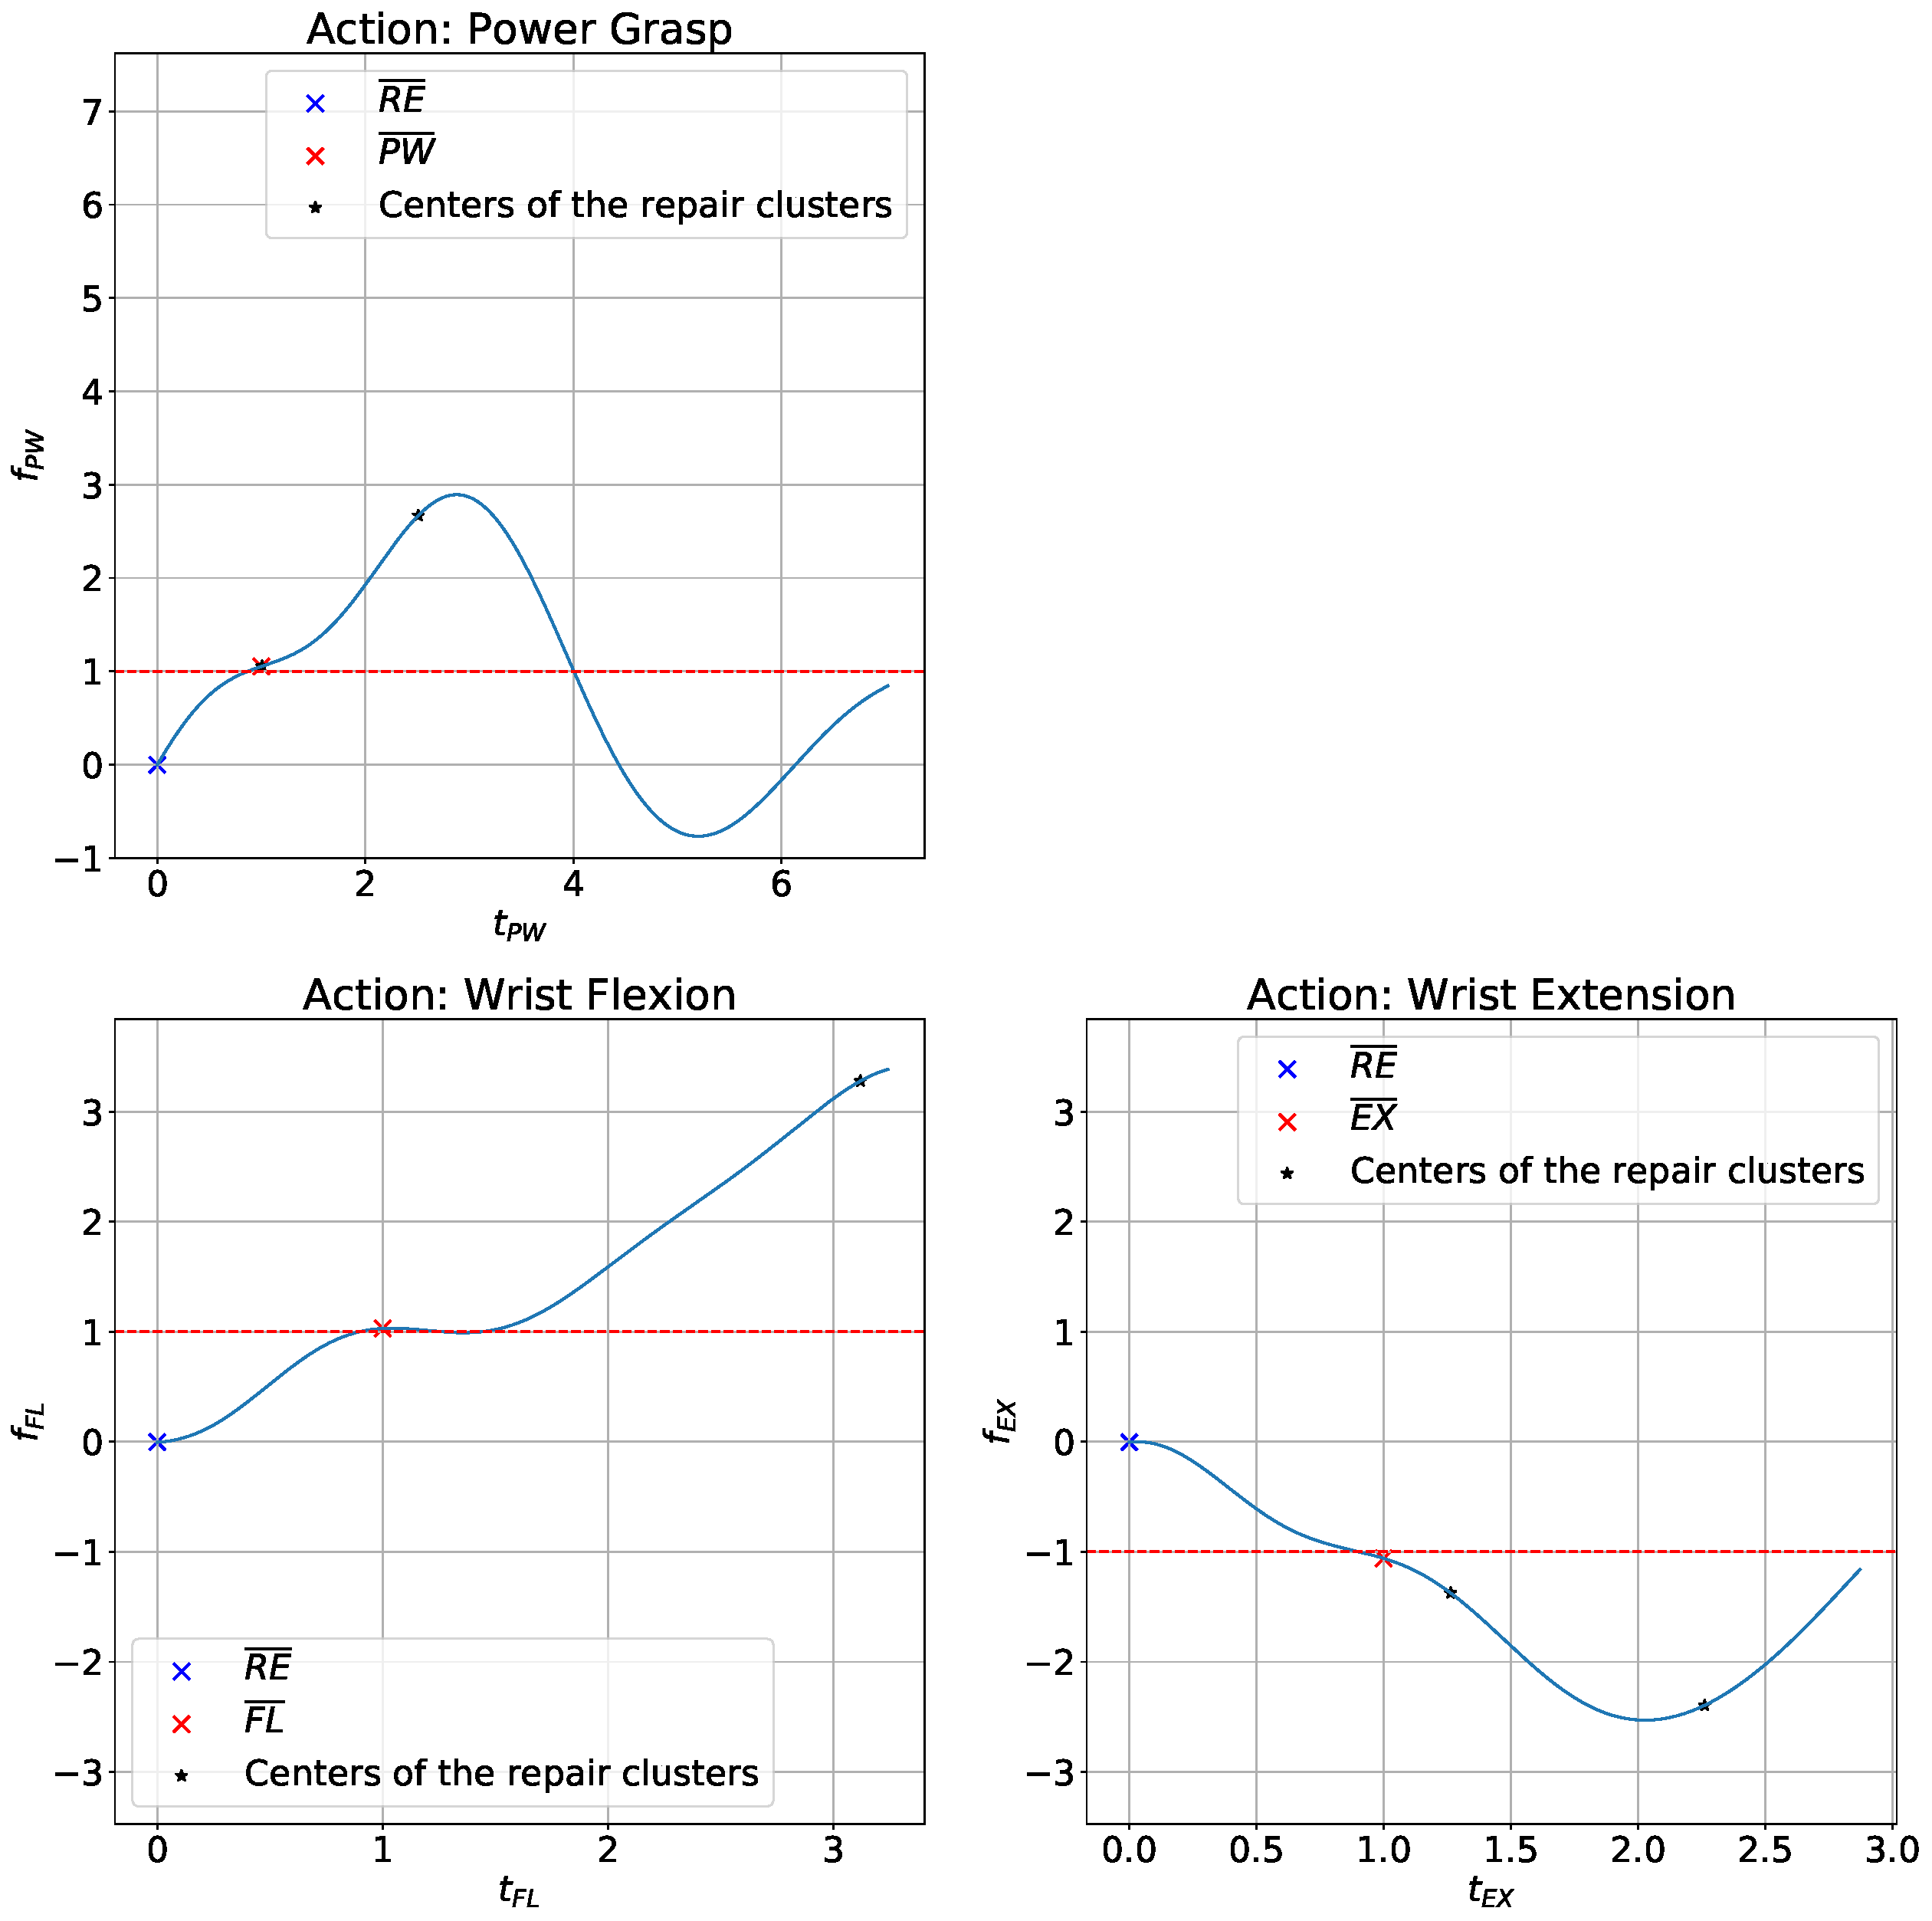
\includegraphics[width=\textwidth]{Images/repair-example/SMT-State2.pdf}
    \caption{In this figure we show the model along the straight lines $\overline{RE} + (\overline{PW} - \overline{RE})t_{PW}$, $\overline{RE} + (\overline{FL} - \overline{RE})t_{FL}$ and $\overline{RE} + (\overline{EX} - \overline{RE})t_{EX}$ after the second round of repair. The red dashed lines represent the maximum activation values for the different actions.}
    \label{fig:SMT-exec-2}
\end{figure}
\begin{figure}[H]
    \centering
    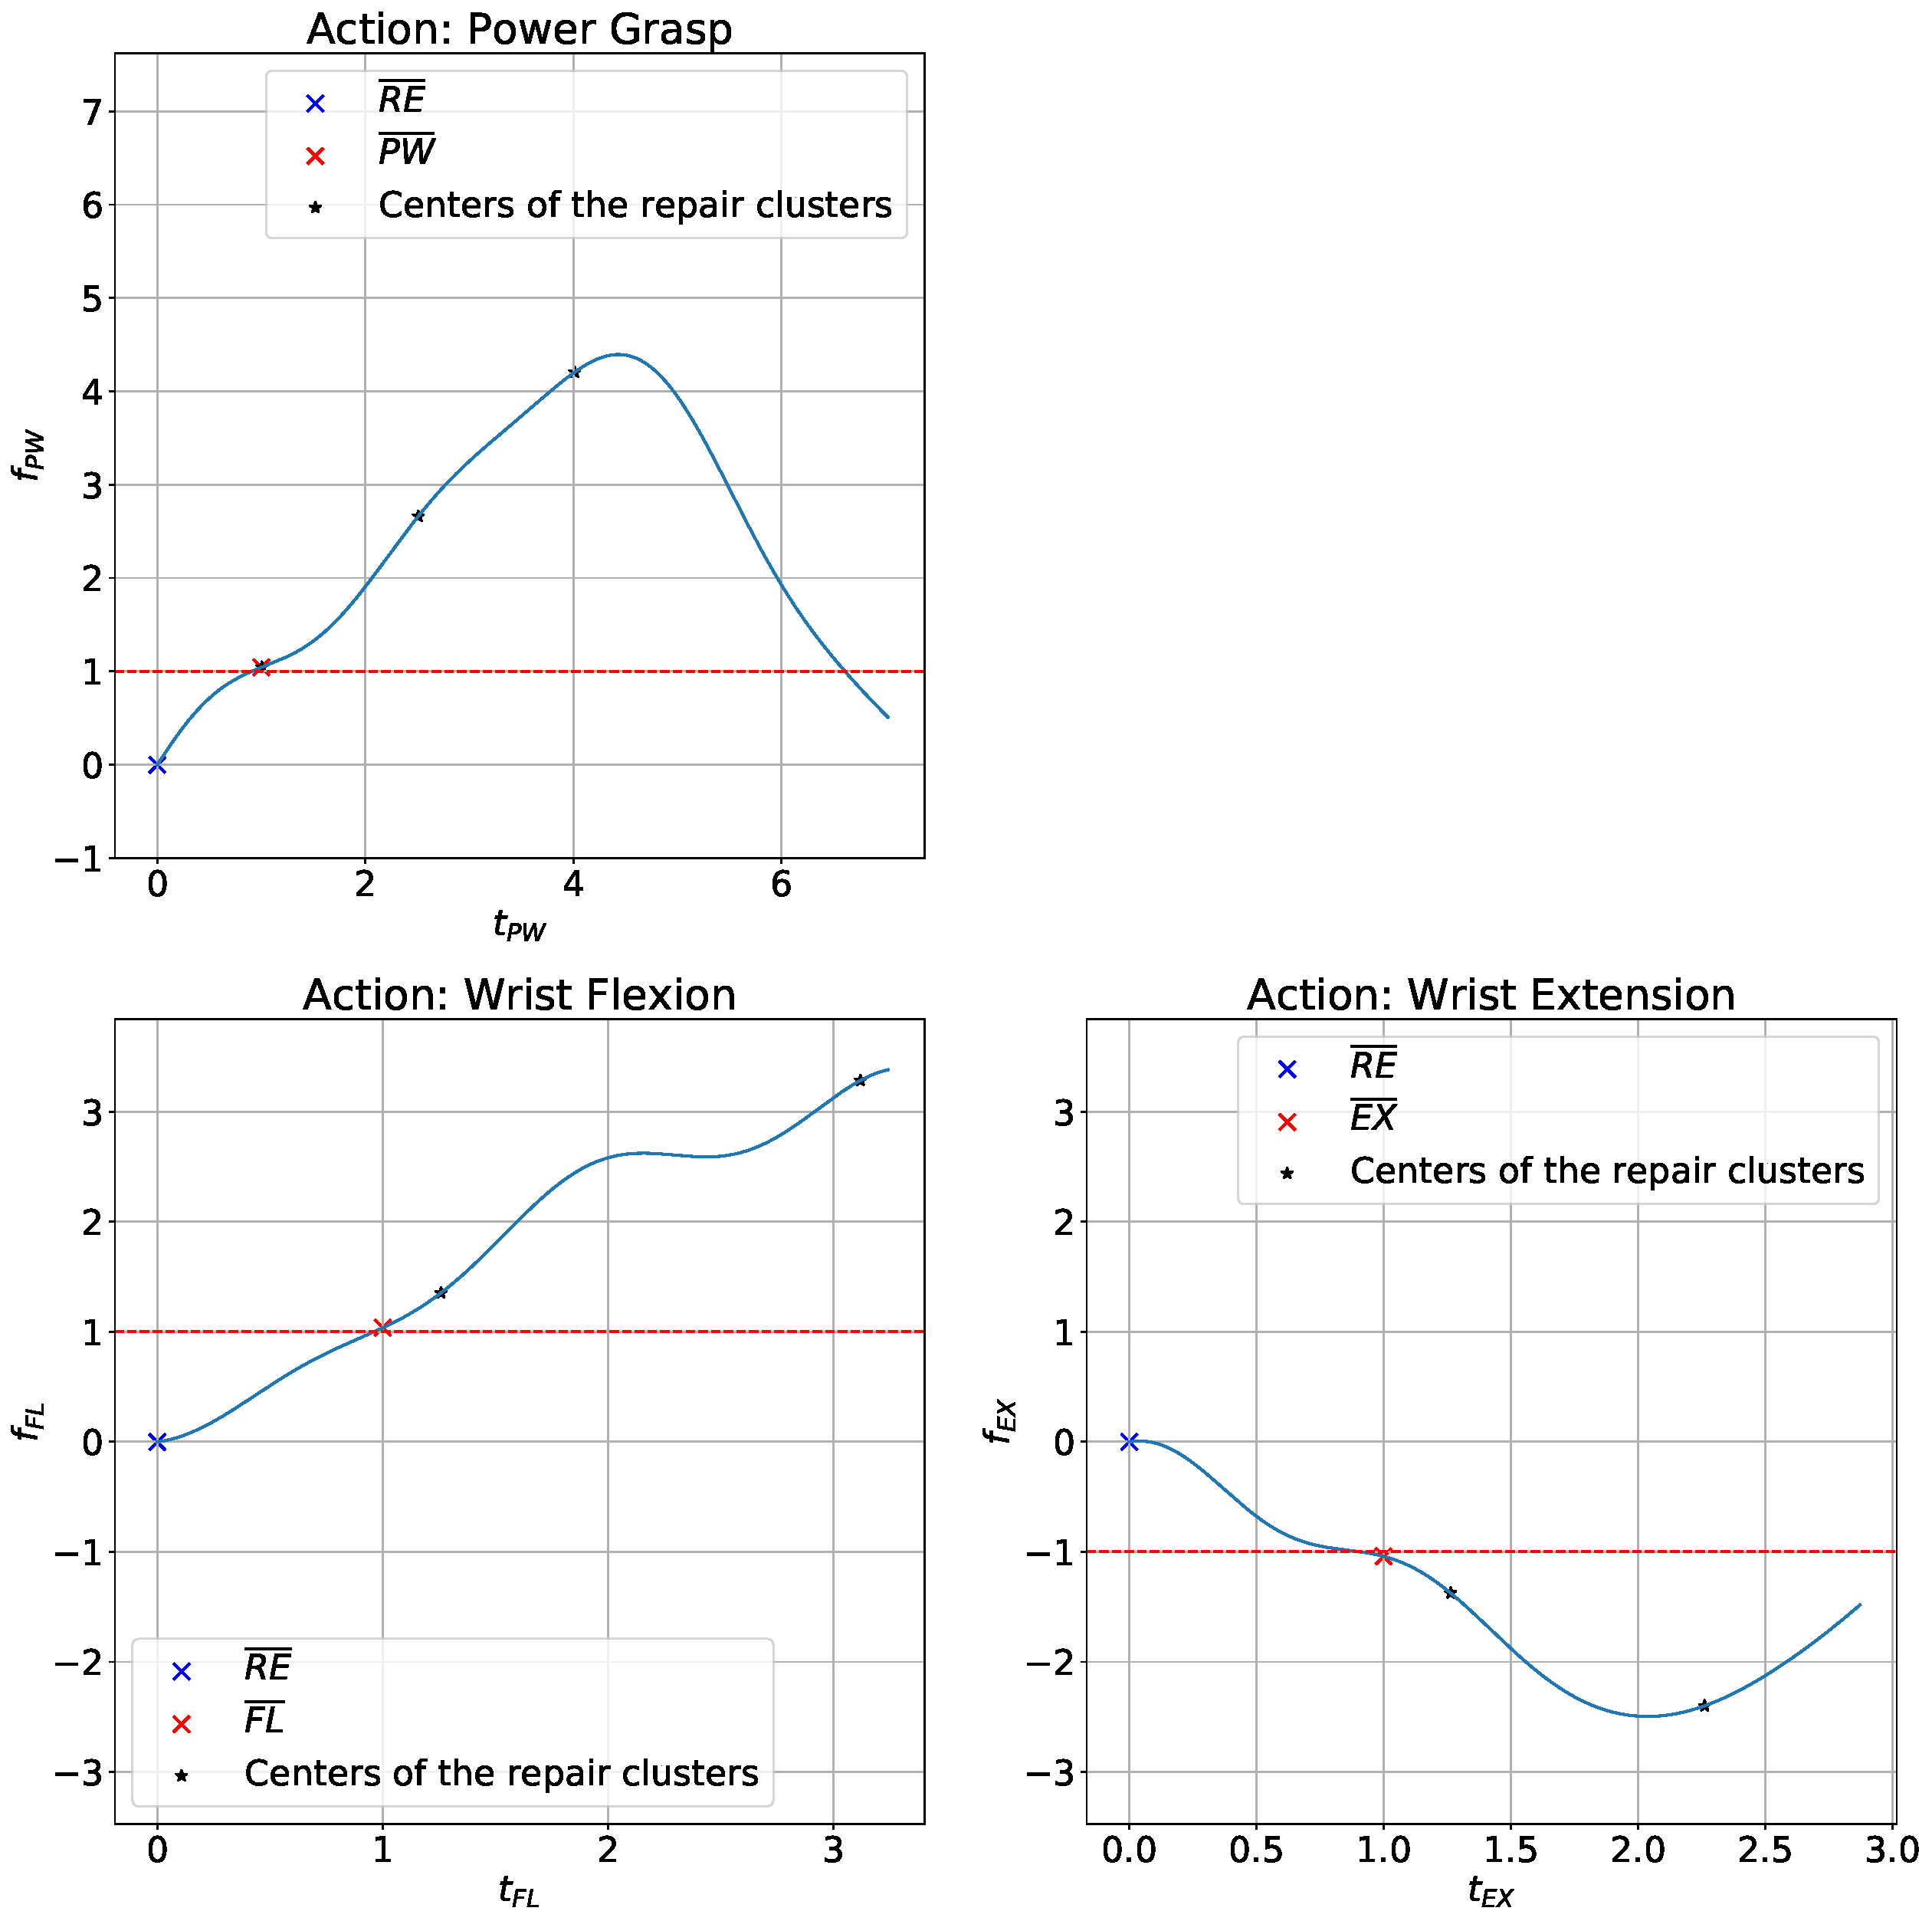
\includegraphics[width=\textwidth]{Images/repair-example/SMT-State3.pdf}
    \caption{In this figure we show the model along the straight lines $\overline{RE} + (\overline{PW} - \overline{RE})t_{PW}$, $\overline{RE} + (\overline{FL} - \overline{RE})t_{FL}$ and $\overline{RE} + (\overline{EX} - \overline{RE})t_{EX}$ after the third round of repair. The red dashed lines represent the maximum activation values for the different actions.}
    \label{fig:SMT-exec-3}
\end{figure}
\begin{figure}[H]
    \centering
    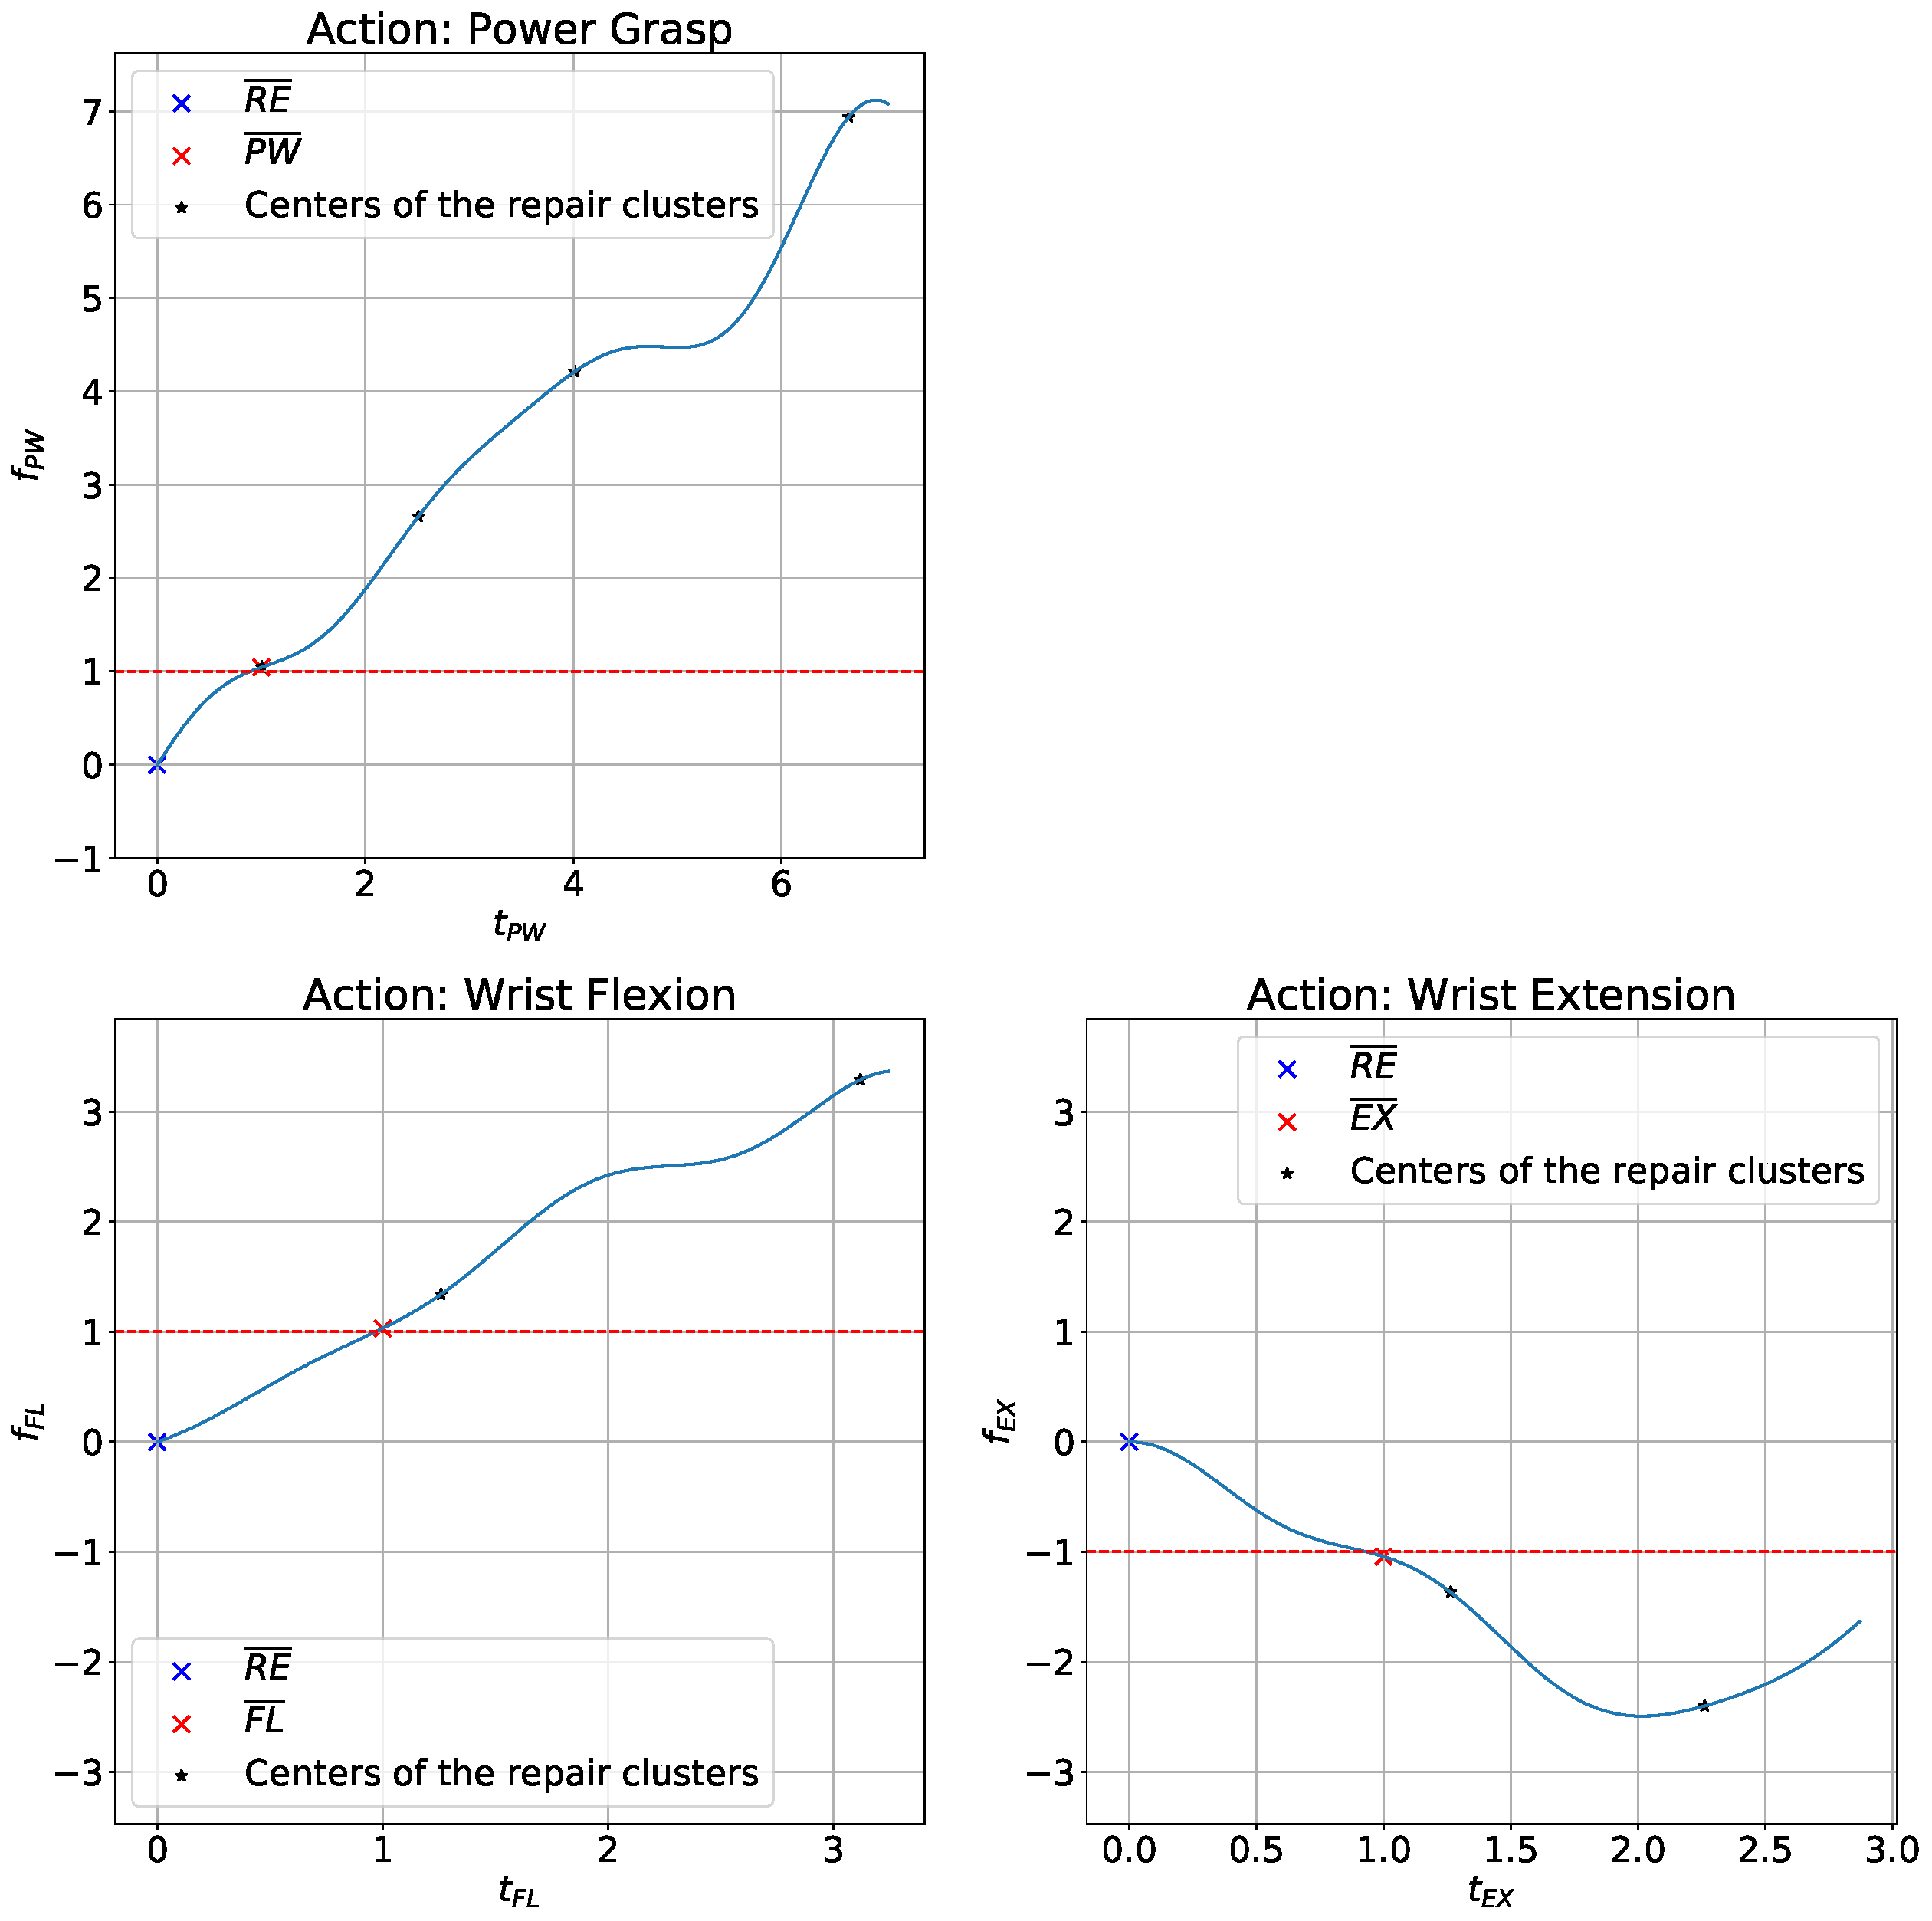
\includegraphics[width=\textwidth]{Images/repair-example/SMT-State4.pdf}
    \caption{In this figure we show the model along the straight lines $\overline{RE} + (\overline{PW} - \overline{RE})t_{PW}$, $\overline{RE} + (\overline{FL} - \overline{RE})t_{FL}$ and $\overline{RE} + (\overline{EX} - \overline{RE})t_{EX}$ after the final round of repair. The red dashed lines represent the maximum activation values for the different actions.}
    \label{fig:SMT-exec-4}
\end{figure}
As can be seen from the figures \ref{fig:PDO-exec-3} and \ref{fig:SMT-exec-4} the final results of the two repair procedures are quite similar and both manage to repair the process till the safety condition is verified (e.g. there are no unsafe points). From the graphs of the two executions can be easily seen one of the difference between the two repair process: since the PDO-Repair always search for the most unsafe points it is usually faster (e.g. require to generate less repair clusters). The other, and most important, difference between the two procedures is that the SMT-Repair guarantee the results to be correct accepting a one sided $\delta$-bounded error on the answer, where $\delta$ is a real positive number we can freely choose. Smaller value of $\delta$ corresponds to an higher computational complexity of the problem and therefore to a longer time necessary to complete the repair process; in particular what requires more time is the $\mathbf{safetyCheck(...)}$ procedure in which the SMT solver is used.
Even if we can guarantee a certain precision also for the PDO-Repair, increasing the number of points we use to analyse the straight lines, it is \textit{impossible to guarantee any level of precision} on the target values whereas the SMT-Repair guarantee a bound, given by $\delta$, on the answers of the SMT solver and therefore on the target values.
\begin{figure}[H]
    \centering
    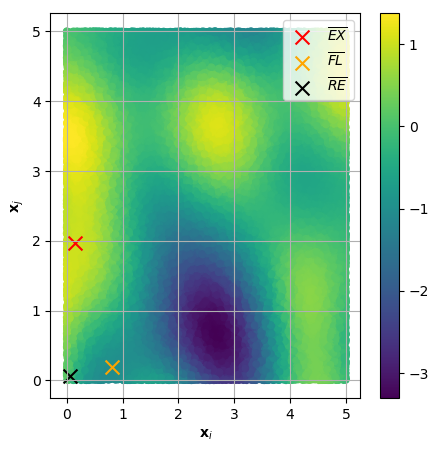
\includegraphics[width=0.45\textwidth]{Images/repair-example/SMT-2D-State0.png}
    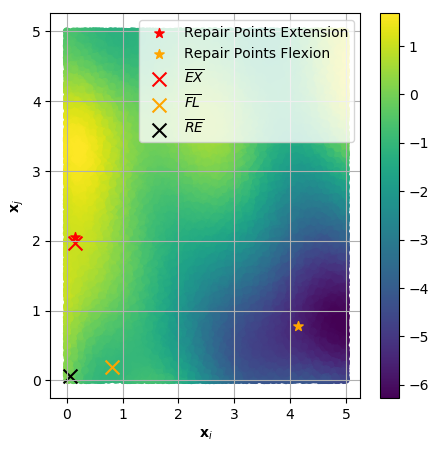
\includegraphics[width=0.45\textwidth]{Images/repair-example/SMT-2D-State1.png}
    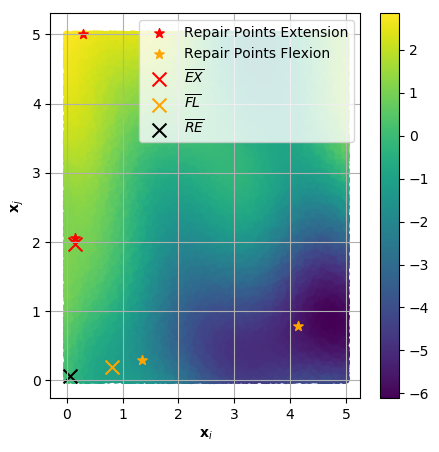
\includegraphics[width=0.45\textwidth]{Images/repair-example/SMT-2D-State2.png}
    \caption{In this figure we show the execution of SMT-Repair on a model built on a 2D-reduced exemplary dataset obtained after gathering observation for three actions (rest, RE; wrist flexion, FL; wrist extension, EX). We chose a 2D reduced dataset in order to be able to show the behaviour of the model on the whole input space.}
    \label{fig:SMT-exec-2D}
\end{figure}
Figure \ref{fig:SMT-exec-2D} shows that, even if our repair process explore only the subset of the input space represented from the straight lines of the type $\overline{RE} + (\overline{A} - \overline{RE})t_{A}$, the characteristics of the learning model guarantee a certain level of continuity which manage to extend the repairing also to the input space that it is not explicitly explored. This kind of generalisation, which we expect to be valid also for the full-dimensionality case, is the reason why the repair process manage to effectively enhance the reliability of the model in the real case, in which we are not only interested in the input space along the straight lines.